\subsection{Blowup Complex}
Like homology, the blowup complex may be defined for arbitrary topological 
spaces~\cite{zc-lh-08}, but in this paper, we focus on blowups of simplicial 
complexes. For a longer exposition of the \mvb{} we refer the reader to Zomorodian
\& Carlsson~\cite{zc-lh-08}. Given a simplicial complex $K$ and cover 
$U = \{U^i\}_i$ of $n$ subcomplexes, let 
$\K^J = \cap_{k \in J} U^j$. The \emph{Mayer-Vietoris blowup complex} is:

\begin{align*}
\K^U &= \bigcup_{\emptyset \not = J \subseteq [n-1]} \K^J \times \Delta^J,
\end{align*}

where $\times$ is the Cartesian product~\cite{zc-lh-08} and $\Delta^J$ is a face of $\N(\C)$.
 % Do example here before any further talk.
\begin{example}
\label{ex:blowup}
Suppose we have a space $\K$ with cover $\C = \{ \C^0, \C^1 \}$ as is shown on 
the top of Figure~\ref{fig:space-n-cover}, where we use a line as a 
representative space and ovals to indicate cover sets, and the four vertices
of the line are labeled from left to right as $a, b, c, d$ respectively.
The cover defines the intersection $\K^{[1]} = \K^{ \{ 0 , 1 \} }$. 
The corresponding blowup is shown in in Figure~\ref{fig:blowup}. We list each of
the relevant pieces of $\K^{\C}$ as well as the nerve of the cover where we denote simplices as strings for 
brevity.  

\begin{align*}
\N(\C) &= \{ 0, 1, 01 \} \\
\K^0 \times \Delta^{\{0\}} &= \{a,b,c,ab,bc\} \times \{0\}, \\
\K^1 \times \Delta^{\{1\}} &= \{b,c,d,bc,bd\} \times \{0\}, \\
\K^{[1]} \times \Delta^{[1]} &=\{b,c,bc\} \times \{01\}. 
\end{align*}

\end{example}
\begin{figure*}
\centering
\subfigure[Space and Cover]{
	\label{fig:space-n-cover}
	\def\svgwidth{1.25in}
	\input{figs/blowup_parts.pdf_tex}
}
\hfill
\subfigure[Local pieces of the blowup complex.]{
	\label{fig:local-pieces}
	\def\svgwidth{1.1in}
	\input{figs/local_pieces.pdf_tex}
}
\hfill
\subfigure[The blowup complex.]{
	\label{fig:blowup}
	\def\svgwidth{1.1in}
	\input{figs/blowup_complex.pdf_tex}
}
%\hfill
%\subfigure[Persistence Barcode. Colors represent homology groups computed
%	   on each piece of the blowup complex. Stacked colors represent 
%  parallelism]{
%	\label{fig:barcode}
%	\def\svgwidth{1.1in}
%	\input{figs/barcode.pdf_tex}
%}
\caption{Our approach. We are given a space equipped with a 
	 cover~\subref{fig:space-n-cover}, the former represented by a path with
         four vertices and three edges and the latter represented by ovals.  
	 First, at time $(t = 0)$ we blowup up the space into 
	 local pieces~\subref{fig:local-pieces}, each local piece is a copy of 
	 the corresponding cover set, then, at $(t = 1)$ we glue together 
	 duplicated simplices by adding in the blowup cells, rendering them 
	 homologically equivalent, which gives us the blowup 
	 complex~\subref{fig:blowup}.
}
\label{fig:vignette}
\end{figure*}

% key property
Our work is based on the following key property.
The blowup complex $\K^U$ has the same homology as its base complex $\K$ in any 
dimension: $H_n(\K^U) \cong H_n(\K)$ for any $n$~\cite[Lemma 1]{zc-lh-08}. 
Our approach then is to compute homology of the blowup complex 
instead of the base complex. The blowup has a structure that allows 
for computation in parallel, unlike the base complex.

% simplicial
To compute the homology of the blowup complex, we may interpret the definition 
above in two different ways.  
At the space level, we may view each cell of the blowup complex as a product 
of two simplices $\sigma \times \Delta^J$, where 
$\sigma \in \K$ and $\Delta^J \in \Delta^n$.  
For example, the product of two edges, $bc \times \{01\}$, gives us a 
quadrilateral cell in Example~\ref{ex:blowup}.  
We may then triangulate the blowup complex to get a simplicial complex in order 
to compute its homology.  While this approach is theoretically correct, it is 
computationally prohibitive in practice due to the need for triangulation and 
unnecessary. We use an alternative interpretation to avoid this work.

% chain
Alternatively, we examine the chain complex attached to the blowup complex.
A basis for $C_n(K^U)$ is the set composed of elements 
$\sigma \tensor \Delta^J$ for all $\emptyset \not = J \subseteq [n-1]$ and 
simplices $\sigma \in K^J$ where $\dim{\sigma} + \dim{\Delta^J} = n$.  
We define the boundary operator as~\cite[\textrm{Lemma }4]{zc-lh-08}:

\begin{align*}
\bd{\left (\sigma \tensor \Delta^J \right)}
&=
\bd{\sigma} \tensor \Delta^J + 
(-1)^{\dim{\sigma}}\sigma \tensor \bd\Delta^J.
\end{align*}

Here, we are defining a boundary operator for the blowup complex on the left 
using the boundary operators on the right, all of which are simplicial and were 
defined in the previous section. 
\begin{example}
The boundary of the quadrilateral cell 
$bc \times \{01\}$: in Example~\ref{ex:blowup} is:

\begin{align*}
\bd{\left (bc \tensor \{01\} \right)}
&=
\bd{(bc)} \tensor \{01\} - bc \tensor \bd(\{01\}) \\
&= c \tensor \{01\} - b \tensor \{01\} - bc \tensor \{1\} + bc \tensor \{0\}.
\end{align*}

\end{example}
Having specified the basis for the chain complex and a boundary operator, 
we now need a filtration on the basis elements in order to use the 
persistence algorithm. In principle an arbitrary filtration will do.
But for computing homology in parallel, we will specify a particular filtration 
whose structure mirrors the structure of the blowup complex. 

\section{Blowup Structure}
\label{sec:blowup_structure}
%intro
The construction of the blowup complex has two phases,  the \emph{local} and the
 \emph{global} phase. In the local phase, the complex explodes into multiple 
pieces, as in Figure~\ref{fig:local-pieces}. This means that we have potentially multiple versions of a simplex 
represented by the various sets in the cover. For example, since edge $bc$ falls within both sets in the 
cover in Figure~\ref{fig:space-n-cover}, it is represented by two cells 
$bc \times 0$ and $bc \times 1$. The pieces at the local stage are disjoint, so 
we may compute the homology of the pieces in parallel. 

The global phase specifies cells that glue the different versions of the 
original simplices together, rendering them homologically equivalent.  
For example, in Figure~\ref{fig:blowup}, the cell 
$b \times 01$ connects $b \times 0$ and $b \times 1$.  

To describe a filtration on the blowup complex, we assume that we have an 
arbitrary filtration $\Filt{\K}$ on the simplices of our input complex $\K$.  In practice, 
we often label the vertices of a complex using numbers or letters and use the lexicographic 
ordering of the vertices to generate a filtration on the complex. We use the same procedure 
with $\N(\C)$ as its vertices are numbered by definition.

Given a filtration $\Filt{\K}$ on $\K$ and $\Filt{\N(\C)}$ on $\Delta^n$ we define a partial order $\Filt{{\K^\C}}$ by 
ordering all cells in the local phase before those in the global phase. This amounts to 
comparing two cells $\sigma \times \Delta^M$ and $\tau \times \Delta^N$ by  
comparing the second factor according to $\Filt{\N(\C)}$. We may complete this partial order to a filtration by then comparing the 
first factor according to $\Filt{\K}$. 
\begin{example}
Figure~\ref{fig:blowup} has the following filtration: 

\begin{equation*}
(\overbrace{a \times 0, b \times 0 ,c \times 0,  ab \times 0, bc \times 0}^
{\textrm{Local Piece \#0 } (t=0)},
\overbrace{b \times 1 , c \times 1, d \times 1, bc \times 1, cd \times 1}^
{\textrm{Local Piece \#1 }(t=0)},
\overbrace{b \times 01, c \times 01, bc \times 01}^
{\textrm{Global Piece } (t=1)}).
\end{equation*}

\end{example}
\begin{figure}
\begin{multicols}{2}
{
\begin{codebox}
\Procname{$\proc{Multicore-Homology}(\K,p)$}
 \li  $\C \gets \proc{Cover}(\K, p)$
 \li  $\K^{\C} \gets \proc{Build-Blowup-Complex}(\K, \C)$
 \li  $\Parfor$   $\Delta^J \in \N(\C)$
 \li  \Do $\proc{Pair-Cells}(\K^{J} \times \Delta^{J})$
      \End
 \li $\For$ $\Delta^J \in \N(\C)$ a $d$-cell for $d > 0$.
 \li  \Do $\proc{Pair-Cells}(\Cl{(\K^{J} \times \Delta^{J})})$ 
\end{codebox}
}
{
\begin{codebox}
\Procname{$\proc{Build-Blowup-Complex}(\K, \C)$}
\li $\K^{\C} \gets \emptyset$
\li $\Parfor$ $\sigma \in \K$
\li \Do $\For$ $\tau \subseteq \C[\sigma]$
\li \Do $\K^{\C} \gets \K^{\C} \cup (\sigma \times \tau)$ 
\end{codebox}
}
\end{multicols}
\caption{Psuedocode for computing the blowup complex and it's homology in parallel. $\proc{Cover}$ can be any algorithm for generating a cover of $\K$ by $p$ subspaces. We encode the cover $\C$ as a map from $\K$ to $\N(\C)$ where each simplex is mapped to the maximal cell in $\N(\C)$ to which it is a member of. The procedure $\proc{Pair-Cells}$ is defined in the Computational Topology section of the Algorithms and Theory of Computation Handbook \cite{z-ct-10}.}
\label{fig:multicore-code}
\end{figure}
Algorithm~\ref{fig:multicore-code} shows how to build the blowup complex and compute it's homology in parallel. The procedure $\proc{Build-Blowup-Complex}$ runs in parallel and has parallel running time $O(2m/p + p)$ time where $m = \card{\K^{\C}}$ and $p$ is the number of processors available. In practice $\proc{Build-Blowup-Complex}$ not only produces a blowup complex but also the filtration of the blowup complex prescribed above. Aside from its output $\proc{Build-Blowup-Complex}$ only uses $O(p)$ extra space. While we have written that the second for-loop in $\proc{Multicore-Homology}$ is to be carried out in serial more parallelism is possible. By ordering the iterations of the loop according to the topology of $\N(\C)$. We leave this added parallelism for future work.
 
The size of the blowup complex depends on the cover. In the worst case, all of 
the simplices in a space $\K$ are contained within all $n$ sets of the cover 
$\C$. In this case, for each simplex $\sigma \in \K$ we have a corresponding 
product cell $\sigma \times \Delta^n$, which has $2^n$ faces. That is, the 
blowup complex \emph{blows up} $\K$ to be $2^n$ times larger, thus deserving 
its name. Therefore, it is imperative to find a cover which minimizes blowup but whose
nerve also allows for parallelism. 

\section{Covers}
\label{sec:covers}
Given a simplicial complex $\K$, our goal is to compute its homology.  
Our approach, as illustrated in Figure~\ref{fig:vignette}, is to find a cover, 
build the associated blowup complex, and compute the homology of the blowup complex in 
parallel. We have now explained all the steps of this approach except how to find a cover. 
We begin in Section~\ref{sec:hardness} by identifying 
properties of covers that lend themselves to efficient computation.
We continue by stating an optimization problem over covers which 
minimizes the explosive size of the blowup of a complex. We then show this optimization problem to be \NPH{}.  
In Section~\ref{sec:partition-based-covers}, we describe an algorithm 
that generates covers which have a simple structure, and bounded overlap 
based on graph partitions. We end this section by showing how a partition of the 
0-cells of a complex can be lifted to a partition of a filtration on the complex 
which can be used to compute homology in parallel without building the blowup complex.
\subsection{Minimum Blowups}
\label{sec:hardness}
In this section, we formalize the problem of finding covers
that minimize blowup size. We show that this problem is \NPH{}, and its 
decision-variant, \NPC{}.

It should be clear that seek a cover which does not yield a large blowup complex. 
To quantify blowup, we define the $\emph{blowup factor}$ as the ratio: 
$\factor.$ We search for a cover $\C$ of size $p$ that minimizes the blowup 
factor. Since we intend to compute the homology of each local piece in parallel,
 the number of local pieces of the blowup should be the number $p$ of available 
processors. Finally, each local piece should be approximately the same 
size. There are many ways of modeling this last constraint. 
We model it by enforcing that no cover set should be larger than a fixed fraction
$\alpha$ of the size of the input complex, where $\alpha \in (1/p,1)$. 
Putting together all of the desired properties of blowups, we have the following 
optimization problem stated for $p = 2$ and $\alpha \in (1/2, 1)$:
\begin{description}
\addtolength{\itemsep}{-.7\baselineskip}
\item[\textsc{Problem:}]  \ablp 
\item[\textsc{Instance:}] A simplicial complex $K$
\item[\textsc{Goal:}] Find a cover $\C$ of $\K$ with $2$ elements such that: 
\[ \max{\card{\C_i}} \leq \alpha\card{\K} \textrm{ and } \factor \textrm{ is minimized.} \]
\end{description}
Our goal is to show that this problem is $\NPH{}$ and it's decision problem variant $\NPC{}$.
For the decision problem variant to be $\NPC{}$ we need to show that $\factor$ may
be evaluated in polynomial time. Recall that $\K^{\C}$ might be exponentially larger than $\K$. 
For covers by two sets we may employ the following lemma.
\begin{lemma}
\label{lem:char-blowup-sol}
Let $\K$ be a complex and let $\C = \{\C_1, \C_2\}$ be a cover of $\K$ 
by two sub complexes. Then:
\begin{equation*}
\factor = 1 + 2\frac{\card{\C_1 \cap \C_2}}{\card{\K}}. 
\end{equation*}
\end{lemma}
\begin{proof}
This follows directly from the product cell definition of $\K^\C$.
\end{proof}
\noindent Now we observe an important necessary condition of optimal solutions to \ablp{}.
\begin{lemma}
\label{lem:blowup-sol-max-simplices}
Given a complex $\K$ and $\C = \{\C_1, \C_2\}$ be an optimal solution of  \ablp{}, then 
$\C$ may be viewed as a partition of $\M(\K)$ the maximal cells of $\K$.
\end{lemma}
\begin{proof}
If $\sigma \in \C_i \cap \C_j$ is a maximal cell, then consider the cover
$\C'$ obtained by removing $\sigma$ from the set of larger
cardinality. $\C'$ is certainly a cover satisfying $\alpha$-balance but
by Lemma~\ref{lem:char-blowup-sol} the blowup factor has decreased
which contradicts the optimality of $\C$.
\end{proof}
\noindent Suppose the input to \ablp{} is a graph $G$. In this context any cover $\C$ of $G$ is a pair of subgraphs $G_1,G_2$.
Lemma~\ref{lem:blowup-sol-max-simplices} tells us that in any optimal solution the intersection $I = G_1 \cap G_2$ of these two 
subgraphs is a set of vertices. The requirement that $\C$ is a cover implies that $I$ is a vertex separator.  \avertex{} is a similar problem on graphs. 
For any $\alpha \in (\frac{1}{2},1)$:
\begin{description}
\addtolength{\itemsep}{-.8\baselineskip}
\item[\textsc{Problem:}]  \avertex{}
\item[\textsc{Instance:}] A graph $G$
\item[\textsc{Goal:}] Find a vertex separator $(V_1,V_2,I)$ of $G$ such that: 
\[ \card{I} \textrm{ is minimized.} \textrm{ subject to } \max_i{(\card{V_i} + \card{E_i})} + \card{I} \leq \alpha(\card{V}+\card{E})  \]
\end{description}
where $E_i$ is the set of edges with at least one endpoint in $V_i$. \avertex{} is \NPH{} for any $\alpha \in (\frac{1}{2},1)$ and it's decision problem variant is \NPC{}~\cite{rhl-yaggpis-14}.
\begin{theorem}
For any $\alpha \in (1/2,1)$ the optimization problem \ablp{}  is \NPH{} and it's decision problem variant \NPC{}.
\end{theorem}
\begin{proof}
We restrict our problem to graph instances of $\avertex{}$ and the problems become equivalent.
\end{proof}
This procedure shows us how finding optimal blowups of graphs finds us a partition of that graph. In the next section we show how given a complex $\K$ 
finding partition of it's 1-skeleton can be used to produce a cover of the entire complex.
\subsection{Partition-Based Covers}
\label{sec:partition-based-covers}
\label{sec:pcover}
\begin{figure*}
\centering
\begin{subfigure}[b]{.24\textwidth}
%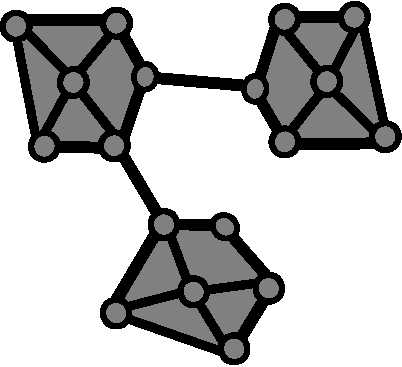
\includegraphics[width=\textwidth]{input_space}
\begin{tikzpicture}[scale=.5,y=-0.80pt, x=0.8pt]
\begin{scope}
\begin{scope}% layer1
    \draw[fill=gray, draw=black,  line width=2]  (142,195) node (a) {} circle (6pt);
    \draw[fill=gray, draw=black,  line width=2]  (95,202) node (b) {} circle (6pt); 
    \draw[fill=gray, draw=black,  line width=2]  (122,155) node (c) {} circle (6pt);  
    \draw[fill=gray, draw=black,  line width=2]  (160,152) node (d) {} circle (6pt);  
     \draw[fill=gray, draw=black,  line width=2]  (170,225)node (e) {}  circle (6pt);  
      \draw[fill=gray, draw=black,  line width=2]  (185,185) node (f) {} circle (6pt);  
      \begin{pgfonlayer}{quadcell}
     \filldraw[color=gray]  (b.center) -- (c.center) -- (d.center) -- (f.center) --  (e.center) -- cycle;
     \end{pgfonlayer}
      \begin{pgfonlayer}{edges}
      \path[color=black, line width=2] (a.center) edge (b.center);
      \path[color=black, line width=2] (a.center) edge (c.center);
      \path[color=black, line width=2] (a.center) edge (d.center);
      \path[color=black, line width=2] (a.center) edge (e.center);
      \path[color=black, line width=2] (a.center) edge (f.center);
      \path[color=black, line width=2] (e.center) edge (f.center) edge (b.center);
      \path[color=black, line width=2] (c.center) edge (b.center) edge (d.center);
       \path[color=black, line width=2] (d.center) edge (f.center);
       \path[color=black, line width =2] (122,155) edge (80, 90);
      \end{pgfonlayer}
\end{scope}
    \begin{scope}[shift={(125,284)},rotate=120]
    \draw[fill=gray, draw=black,  line width=2]  (142,195) node (a) {} circle (6pt);
    \draw[fill=gray, draw=black,  line width=2]  (95,202) node (b) {} circle (6pt); 
    \draw[fill=gray, draw=black,  line width=2]  (122,155) node (c) {} circle (6pt);  
    \draw[fill=gray, draw=black,  line width=2]  (160,152) node (d) {} circle (6pt);  
     \draw[fill=gray, draw=black,  line width=2]  (170,225)node (e) {}  circle (6pt);  
      \draw[fill=gray, draw=black,  line width=2]  (185,185) node (f) {} circle (6pt);  
      \begin{pgfonlayer}{quadcell}
     \filldraw[color=gray]  (b.center) -- (c.center) -- (d.center) -- (f.center) --  (e.center) -- cycle;
     \end{pgfonlayer}
      \begin{pgfonlayer}{edges}
      \path[color=black, line width=2] (a.center) edge (b.center);
      \path[color=black, line width=2] (a.center) edge (c.center);
      \path[color=black, line width=2] (a.center) edge (d.center);
      \path[color=black, line width=2] (a.center) edge (e.center);
      \path[color=black, line width=2] (a.center) edge (f.center);
      \path[color=black, line width=2] (e.center) edge (f.center) edge (b.center);
      \path[color=black, line width=2] (c.center) edge (b.center) edge (d.center);
       \path[color=black, line width=2] (d.center) edge (f.center);
          \path[color=black, line width =2] (160, 152) edge (200, 90);
      \end{pgfonlayer}
                \end{scope}
        \begin{scope}[shift={(198,-138)},rotate=-70]
    \draw[fill=gray, draw=black,  line width=2]  (142,195) node (a) {} circle (6pt);
    \draw[fill=gray, draw=black,  line width=2]  (95,202) node (b) {} circle (6pt); 
    \draw[fill=gray, draw=black,  line width=2]  (122,155) node (c) {} circle (6pt);  
    \draw[fill=gray, draw=black,  line width=2]  (160,152) node (d) {} circle (6pt);  
     \draw[fill=gray, draw=black,  line width=2]  (170,225)node (e) {}  circle (6pt);  
      \draw[fill=gray, draw=black,  line width=2]  (185,185) node (f) {} circle (6pt);  
      \begin{pgfonlayer}{quadcell}
     \filldraw[color=gray]  (b.center) -- (c.center) -- (d.center) -- (f.center) --  (e.center) -- cycle;
     \end{pgfonlayer}
           \begin{pgfonlayer}{edges}
      \path[color=black, line width=2] (a.center) edge (b.center);
      \path[color=black, line width=2] (a.center) edge (c.center);
      \path[color=black, line width=2] (a.center) edge (d.center);
      \path[color=black, line width=2] (a.center) edge (e.center);
      \path[color=black, line width=2] (a.center) edge (f.center);
      \path[color=black, line width=2] (e.center) edge (f.center) edge (b.center);
      \path[color=black, line width=2] (c.center) edge (b.center) edge (d.center);
       \path[color=black, line width=2] (d.center) edge (f.center);
      \end{pgfonlayer}
         \end{scope}
  \end{scope}
\end{tikzpicture}
\caption{Input Complex $\K$}
\label{fig:input}
\end{subfigure}
\hfill
\begin{subfigure}[b]{.24\textwidth}
\begin{tikzpicture}[scale=.5,y=-0.80pt, x=0.8pt]
\begin{scope}% layer1
    \draw[fill=afrapurple, draw=black,  line width=1]  (142,195) node (a) {} circle (6pt);
    \draw[fill=afrapurple, draw=black,  line width=1]  (95,202) node (b) {} circle (6pt); 
    \draw[fill=afrapurple, draw=black,  line width=1]  (122,155) node (c) {} circle (6pt);  
    \draw[fill=afrapurple, draw=black,  line width=1]  (160,152) node (d) {} circle (6pt);  
     \draw[fill=afrapurple, draw=black,  line width=1]  (170,225)node (e) {}  circle (6pt);  
      \draw[fill=afrapurple, draw=black,  line width=1]  (185,185) node (f) {} circle (6pt);  
    \begin{scope}% g10596
      % path7778
      \path[draw=afrapurplelight,line join=miter,line cap=butt,miter limit=4.00,line
        width=2] (142.8068,141.8195) .. controls (140.5229,140.7866) and
        (138.2447,139.7410) .. (135.9724,138.6829) .. controls (133.0686,137.3306) and
        (130.1306,135.9436) .. (126.9750,135.3928) .. controls (123.2061,134.7350) and
        (119.2405,135.3312) .. (115.7977,137.0000) .. controls (112.3550,138.6687) and
        (109.4446,141.3929) .. (107.4859,144.6794) .. controls (105.5194,147.9789) and
        (104.5226,151.7563) .. (103.6919,155.5065) .. controls (102.8612,159.2568) and
        (102.1647,163.0652) .. (100.7192,166.6240) .. controls (98.5492,171.9661) and
        (94.7943,176.4976) .. (90.9055,180.7549) .. controls (87.1005,184.9204) and
        (83.0614,188.9825) .. (80.3662,193.9388) .. controls (79.0186,196.4170) and
        (78.0238,199.1093) .. (77.6619,201.9068) .. controls (77.2999,204.7044) and
        (77.5891,207.6123) .. (78.7040,210.2036) .. controls (79.9202,213.0305) and
        (82.0576,215.3721) .. (84.4182,217.3464) .. controls (89.4627,221.5653) and
        (95.5940,224.2926) .. (101.8472,226.3281) .. controls (108.1004,228.3635) and
        (114.5437,229.7569) .. (120.8468,231.6321) .. controls (125.8989,233.1351) and
        (130.8532,234.9453) .. (135.8468,236.6321) .. controls (143.5496,239.2340) and
        (151.4656,241.5630) .. (159.5933,241.7724) .. controls (167.7210,241.9818) and
        (176.1768,239.8661) .. (182.2754,234.4893) .. controls (186.9397,230.3769) and
        (189.9191,224.6670) .. (192.0037,218.8085) .. controls (194.0883,212.9500) and
        (195.3761,206.8390) .. (197.2754,200.9178) .. controls (198.3603,197.5357) and
        (199.6460,194.2112) .. (200.4716,190.7566) .. controls (201.2972,187.3020) and
        (201.6504,183.6634) .. (200.8468,180.2036) .. controls (200.0756,176.8833) and
        (198.2661,173.8691) .. (196.0175,171.3074) .. controls (193.7689,168.7456) and
        (191.0857,166.6035) .. (188.3386,164.5855) .. controls (182.8445,160.5494) and
        (176.8474,156.7588) .. (173.3140,150.9287) .. controls (171.6874,148.2446) and
        (170.6556,145.2291) .. (168.9715,142.5808) .. controls (168.1294,141.2566) and
        (167.1180,140.0232) .. (165.8705,139.0712) .. controls (164.6230,138.1193) and
        (163.1264,137.4584) .. (161.5611,137.3464) .. controls (160.3978,137.2632) and
        (159.2270,137.4826) .. (158.1251,137.8650) .. controls (157.0233,138.2474) and
        (155.9841,138.7900) .. (154.9709,139.3678) .. controls (152.9447,140.5234) and
        (150.9545,141.8488) .. (148.6798,142.3654) .. controls (146.7303,142.8081) and
        (144.6414,142.6140) .. (142.8068,141.8195);
    \end{scope}
        
    \begin{scope}[shift={(125,284)},rotate=120]
    \draw[fill=afragreen,draw=black,  line width=1]  (142,195) node (a) {} circle (6pt);
    \draw[fill=afragreen, draw=black,  line width=1]  (95,202) node (b) {} circle (6pt); 
    \draw[fill=afragreen, draw=black,  line width=1]  (122,155) node (c) {} circle (6pt);  
    \draw[fill=afragreen, draw=black,  line width=1]  (160,152) node (d) {} circle (6pt);  
     \draw[fill=afragreen, draw=black,  line width=1]  (170,225)node (e) {}  circle (6pt);  
      \draw[fill=afragreen, draw=black,  line width=1]  (185,185) node (f) {} circle (6pt);  
                \end{scope}
    \begin{scope}% g10596
      % path7778
            % path7778-9
      \path[draw=afragreenlight,line join=miter,line cap=butt,miter limit=4.00,line
        width=2] (192.9926,11.9341) .. controls (188.8896,12.6152) and
        (184.9965,14.4282) .. (181.7524,17.0311) .. controls (178.5084,19.6340) and
        (175.9104,23.0138) .. (174.1113,26.7637) .. controls (169.8923,35.5570) and
        (170.1687,45.8307) .. (167.1178,55.0943) .. controls (165.7925,59.1182) and
        (163.8223,63.0319) .. (163.6387,67.2645) .. controls (163.5263,69.8555) and
        (164.1014,72.4453) .. (165.0598,74.8551) .. controls (166.0182,77.2650) and
        (167.3530,79.5081) .. (168.7982,81.6615) .. controls (171.6886,85.9684) and
        (175.0752,90.0199) .. (177.0385,94.8209) .. controls (177.8932,96.9111) and
        (178.4609,99.1056) .. (179.1934,101.2417) .. controls (179.9259,103.3778) and
        (180.8444,105.4903) .. (182.2959,107.2203) .. controls (183.6446,108.8277) and
        (185.4163,110.0510) .. (187.3327,110.9055) .. controls (189.2491,111.7601) and
        (191.3102,112.2567) .. (193.3884,112.5466) .. controls (197.5448,113.1264) and
        (201.7732,112.8927) .. (205.9513,113.2866) .. controls (211.2015,113.7817) and
        (216.3028,115.2594) .. (221.4846,116.2387) .. controls (229.3108,117.7177) and
        (237.3906,118.0536) .. (245.2523,116.7765) .. controls (253.1139,115.4994) and
        (260.7551,112.5790) .. (267.2111,107.9146) .. controls (272.7152,103.9381) and
        (277.3945,98.5796) .. (279.6336,92.1691) .. controls (280.7532,88.9639) and
        (281.2461,85.5266) .. (280.9380,82.1454) .. controls (280.6298,78.7643) and
        (279.5090,75.4439) .. (277.5935,72.6407) .. controls (274.9928,68.8349) and
        (271.0961,66.1511) .. (267.3573,63.4550) .. controls (263.6185,60.7588) and
        (259.8383,57.8362) .. (257.6523,53.7779) .. controls (255.1375,49.1092) and
        (255.0539,43.5530) .. (255.1757,38.2515) .. controls (255.2975,32.9500) and
        (255.5337,27.4624) .. (253.5453,22.5464) .. controls (252.0356,18.8141) and
        (249.2746,15.6239) .. (245.8724,13.4712) .. controls (242.4702,11.3185) and
        (238.4491,10.1936) .. (234.4237,10.1225) .. controls (228.1091,10.0111) and
        (222.0000,12.4065) .. (215.6949,12.7688) .. controls (208.1147,13.2044) and
        (200.4828,10.6908) .. (192.9926,11.9341);
    \end{scope}
        \begin{scope}[shift={(198,-138)},rotate=-70]
    \draw[fill=afrablue, draw=black,  line width=1]  (142,195) node (a) {} circle (6pt);
    \draw[fill=afrablue,draw=black,  line width=1]  (95,202) node (b) {} circle (6pt); 
    \draw[fill=afrablue, draw=black,  line width=1]  (122,155) node (c) {} circle (6pt);  
    \draw[fill=afrablue, draw=black,  line width=1]  (160,152) node (d) {} circle (6pt);  
     \draw[fill=afrablue, draw=black,  line width=1]  (170,225)node (e) {}  circle (6pt);  
      \draw[fill=afrablue, draw=black,  line width=1]  (185,185) node (f) {} circle (6pt);  
         \end{scope}
    \begin{scope}% g10596
      % path7778-4
      \path[draw=afrabluedark,line join=miter,line cap=butt,miter limit=4.00,line
        width=2] (114.2167,41.2393) .. controls (111.5795,35.7883) and
        (110.3171,29.7694) .. (107.8770,24.2274) .. controls (106.6569,21.4563) and
        (105.1297,18.7930) .. (103.0913,16.5543) .. controls (101.0528,14.3156) and
        (98.4767,12.5121) .. (95.5673,11.6741) .. controls (93.1997,10.9921) and
        (90.6823,10.9636) .. (88.2376,11.2700) .. controls (85.7928,11.5764) and
        (83.4024,12.2091) .. (81.0192,12.8346) .. controls (78.6361,13.4602) and
        (76.2421,14.0821) .. (73.7946,14.3663) .. controls (71.3472,14.6505) and
        (68.8282,14.5876) .. (66.4734,13.8627) .. controls (64.2730,13.1855) and
        (62.2883,11.9568) .. (60.3633,10.6941) .. controls (58.4383,9.4313) and
        (56.5283,8.1123) .. (54.4053,7.2216) .. controls (51.6098,6.0489) and
        (48.5082,5.6617) .. (45.4923,5.9694) .. controls (42.4764,6.2771) and
        (39.5466,7.2678) .. (36.8902,8.7284) .. controls (31.5772,11.6495) and
        (27.4415,16.3672) .. (24.2232,21.5057) .. controls (22.6382,24.0364) and
        (21.2430,26.7025) .. (20.3036,29.5370) .. controls (18.2838,35.6312) and
        (18.4521,42.2521) .. (19.4464,48.5949) .. controls (20.4406,54.9377) and
        (22.2309,61.1289) .. (23.4110,67.4398) .. controls (24.3531,72.4776) and
        (24.9041,77.5791) .. (25.4838,82.6714) .. controls (26.3970,90.6930) and
        (27.4212,98.8460) .. (30.7141,106.2174) .. controls (32.3605,109.9031) and
        (34.5756,113.3615) .. (37.4426,116.2032) .. controls (40.3097,119.0448) and
        (43.8461,121.2553) .. (47.7398,122.3203) .. controls (53.5513,123.9098) and
        (59.7541,122.8914) .. (65.5662,121.3043) .. controls (71.3782,119.7172) and
        (77.0782,117.5626) .. (83.0613,116.8547) .. controls (86.5271,116.4447) and
        (90.0380,116.5279) .. (93.5015,116.0988) .. controls (96.9650,115.6697) and
        (100.4817,114.6656) .. (103.1342,112.3975) .. controls (104.6594,111.0933) and
        (105.8396,109.4167) .. (106.7141,107.6106) .. controls (107.5886,105.8044) and
        (108.1667,103.8674) .. (108.6010,101.9082) .. controls (109.4697,97.9899) and
        (109.7788,93.9469) .. (110.9329,90.1030) .. controls (112.5367,84.7609) and
        (115.6923,80.0478) .. (118.3166,75.1262) .. controls (119.6288,72.6653) and
        (120.8193,70.1251) .. (121.6073,67.4499) .. controls (122.3953,64.7747) and
        (122.7732,61.9521) .. (122.4431,59.1829) .. controls (122.0511,55.8942) and
        (120.6821,52.7996) .. (119.0883,49.8963) .. controls (117.4945,46.9930) and
        (115.6592,44.2207) .. (114.2167,41.2393);
    \end{scope}
  \end{scope}
\end{tikzpicture}
\caption{Partition $P$}
\label{fig:part}
\end{subfigure}
\hfill
\begin{subfigure}[b]{.24\textwidth}
\begin{tikzpicture}[scale=.5,y=-0.80pt, x=0.8pt]
\begin{scope}

\begin{scope}% layer1
    \draw[fill=afrapurple, draw=afrapurpledark,  line width=2]  (142,195) node (a) {} circle (6pt);
    \draw[fill=afrapurple, draw=afrapurpledark,  line width=2]  (95,202) node (b) {} circle (6pt); 
    \draw[fill=afrapurple, draw=afrapurpledark,  line width=2]  (122,155) node (c) {} circle (6pt);  
    \draw[fill=afrapurple, draw=afrapurpledark,  line width=2]  (160,152) node (d) {} circle (6pt);  
     \draw[fill=afrapurple, draw=afrapurpledark,  line width=2]  (170,225)node (e) {}  circle (6pt);  
      \draw[fill=afrapurple, draw=afrapurpledark,  line width=2]  (185,185) node (f) {} circle (6pt);  
      \begin{pgfonlayer}{quadcell}
     \filldraw[color=afrapurple]  (b.center) -- (c.center) -- (d.center) -- (f.center) --  (e.center) -- cycle;
     \end{pgfonlayer}
      \begin{pgfonlayer}{edges}
      \path[color=afrapurpledark, line width=2] (a.center) edge (b.center);
      \path[color=afrapurpledark, line width=2] (a.center) edge (c.center);
      \path[color=afrapurpledark, line width=2] (a.center) edge (d.center);
      \path[color=afrapurpledark, line width=2] (a.center) edge (e.center);
      \path[color=afrapurpledark, line width=2] (a.center) edge (f.center);
      \path[color=afrapurpledark, line width=2] (e.center) edge (f.center) edge (b.center);
      \path[color=afrapurpledark, line width=2] (c.center) edge (b.center) edge (d.center);
       \path[color=afrapurpledark, line width=2] (d.center) edge (f.center);
       \path[color=gray, line width =2] (122,155) edge (80, 90);
      \end{pgfonlayer}
    \begin{scope}% g10596
      % path7778
      \path[draw=afrapurplelight,line join=miter,line cap=butt,miter limit=4.00,line
        width=2] (142.8068,141.8195) .. controls (140.5229,140.7866) and
        (138.2447,139.7410) .. (135.9724,138.6829) .. controls (133.0686,137.3306) and
        (130.1306,135.9436) .. (126.9750,135.3928) .. controls (123.2061,134.7350) and
        (119.2405,135.3312) .. (115.7977,137.0000) .. controls (112.3550,138.6687) and
        (109.4446,141.3929) .. (107.4859,144.6794) .. controls (105.5194,147.9789) and
        (104.5226,151.7563) .. (103.6919,155.5065) .. controls (102.8612,159.2568) and
        (102.1647,163.0652) .. (100.7192,166.6240) .. controls (98.5492,171.9661) and
        (94.7943,176.4976) .. (90.9055,180.7549) .. controls (87.1005,184.9204) and
        (83.0614,188.9825) .. (80.3662,193.9388) .. controls (79.0186,196.4170) and
        (78.0238,199.1093) .. (77.6619,201.9068) .. controls (77.2999,204.7044) and
        (77.5891,207.6123) .. (78.7040,210.2036) .. controls (79.9202,213.0305) and
        (82.0576,215.3721) .. (84.4182,217.3464) .. controls (89.4627,221.5653) and
        (95.5940,224.2926) .. (101.8472,226.3281) .. controls (108.1004,228.3635) and
        (114.5437,229.7569) .. (120.8468,231.6321) .. controls (125.8989,233.1351) and
        (130.8532,234.9453) .. (135.8468,236.6321) .. controls (143.5496,239.2340) and
        (151.4656,241.5630) .. (159.5933,241.7724) .. controls (167.7210,241.9818) and
        (176.1768,239.8661) .. (182.2754,234.4893) .. controls (186.9397,230.3769) and
        (189.9191,224.6670) .. (192.0037,218.8085) .. controls (194.0883,212.9500) and
        (195.3761,206.8390) .. (197.2754,200.9178) .. controls (198.3603,197.5357) and
        (199.6460,194.2112) .. (200.4716,190.7566) .. controls (201.2972,187.3020) and
        (201.6504,183.6634) .. (200.8468,180.2036) .. controls (200.0756,176.8833) and
        (198.2661,173.8691) .. (196.0175,171.3074) .. controls (193.7689,168.7456) and
        (191.0857,166.6035) .. (188.3386,164.5855) .. controls (182.8445,160.5494) and
        (176.8474,156.7588) .. (173.3140,150.9287) .. controls (171.6874,148.2446) and
        (170.6556,145.2291) .. (168.9715,142.5808) .. controls (168.1294,141.2566) and
        (167.1180,140.0232) .. (165.8705,139.0712) .. controls (164.6230,138.1193) and
        (163.1264,137.4584) .. (161.5611,137.3464) .. controls (160.3978,137.2632) and
        (159.2270,137.4826) .. (158.1251,137.8650) .. controls (157.0233,138.2474) and
        (155.9841,138.7900) .. (154.9709,139.3678) .. controls (152.9447,140.5234) and
        (150.9545,141.8488) .. (148.6798,142.3654) .. controls (146.7303,142.8081) and
        (144.6414,142.6140) .. (142.8068,141.8195);
    \end{scope}
        \end{scope}
        
    \begin{scope}[shift={(125,284)},rotate=120]
    \draw[fill=afragreen, draw=afragreendark,  line width=2]  (142,195) node (a) {} circle (6pt);
    \draw[fill=afragreen, draw=afragreendark,  line width=2]  (95,202) node (b) {} circle (6pt); 
    \draw[fill=afragreen, draw=afragreendark,  line width=2]  (122,155) node (c) {} circle (6pt);  
    \draw[fill=afragreen, draw=afragreendark,  line width=2]  (160,152) node (d) {} circle (6pt);  
     \draw[fill=afragreen, draw=afragreendark,  line width=2]  (170,225)node (e) {}  circle (6pt);  
      \draw[fill=afragreen, draw=afragreendark,  line width=2]  (185,185) node (f) {} circle (6pt);  
      \begin{pgfonlayer}{quadcell}
     \filldraw[color=afragreen]  (b.center) -- (c.center) -- (d.center) -- (f.center) --  (e.center) -- cycle;
     \end{pgfonlayer}
      \begin{pgfonlayer}{edges}
      \path[color=afragreendark, line width=2] (a.center) edge (b.center);
      \path[color=afragreendark, line width=2] (a.center) edge (c.center);
      \path[color=afragreendark, line width=2] (a.center) edge (d.center);
      \path[color=afragreendark, line width=2] (a.center) edge (e.center);
      \path[color=afragreendark, line width=2] (a.center) edge (f.center);
      \path[color=afragreendark, line width=2] (e.center) edge (f.center) edge (b.center);
      \path[color=afragreendark, line width=2] (c.center) edge (b.center) edge (d.center);
       \path[color=afragreendark, line width=2] (d.center) edge (f.center);
          \path[color=gray, line width =2] (160, 152) edge (200, 90);
      \end{pgfonlayer}
                \end{scope}
    \begin{scope}% g10596
      % path7778
            % path7778-9
      \path[draw=afragreenlight,line join=miter,line cap=butt,miter limit=4.00,line
        width=2] (192.9926,11.9341) .. controls (188.8896,12.6152) and
        (184.9965,14.4282) .. (181.7524,17.0311) .. controls (178.5084,19.6340) and
        (175.9104,23.0138) .. (174.1113,26.7637) .. controls (169.8923,35.5570) and
        (170.1687,45.8307) .. (167.1178,55.0943) .. controls (165.7925,59.1182) and
        (163.8223,63.0319) .. (163.6387,67.2645) .. controls (163.5263,69.8555) and
        (164.1014,72.4453) .. (165.0598,74.8551) .. controls (166.0182,77.2650) and
        (167.3530,79.5081) .. (168.7982,81.6615) .. controls (171.6886,85.9684) and
        (175.0752,90.0199) .. (177.0385,94.8209) .. controls (177.8932,96.9111) and
        (178.4609,99.1056) .. (179.1934,101.2417) .. controls (179.9259,103.3778) and
        (180.8444,105.4903) .. (182.2959,107.2203) .. controls (183.6446,108.8277) and
        (185.4163,110.0510) .. (187.3327,110.9055) .. controls (189.2491,111.7601) and
        (191.3102,112.2567) .. (193.3884,112.5466) .. controls (197.5448,113.1264) and
        (201.7732,112.8927) .. (205.9513,113.2866) .. controls (211.2015,113.7817) and
        (216.3028,115.2594) .. (221.4846,116.2387) .. controls (229.3108,117.7177) and
        (237.3906,118.0536) .. (245.2523,116.7765) .. controls (253.1139,115.4994) and
        (260.7551,112.5790) .. (267.2111,107.9146) .. controls (272.7152,103.9381) and
        (277.3945,98.5796) .. (279.6336,92.1691) .. controls (280.7532,88.9639) and
        (281.2461,85.5266) .. (280.9380,82.1454) .. controls (280.6298,78.7643) and
        (279.5090,75.4439) .. (277.5935,72.6407) .. controls (274.9928,68.8349) and
        (271.0961,66.1511) .. (267.3573,63.4550) .. controls (263.6185,60.7588) and
        (259.8383,57.8362) .. (257.6523,53.7779) .. controls (255.1375,49.1092) and
        (255.0539,43.5530) .. (255.1757,38.2515) .. controls (255.2975,32.9500) and
        (255.5337,27.4624) .. (253.5453,22.5464) .. controls (252.0356,18.8141) and
        (249.2746,15.6239) .. (245.8724,13.4712) .. controls (242.4702,11.3185) and
        (238.4491,10.1936) .. (234.4237,10.1225) .. controls (228.1091,10.0111) and
        (222.0000,12.4065) .. (215.6949,12.7688) .. controls (208.1147,13.2044) and
        (200.4828,10.6908) .. (192.9926,11.9341);
    \end{scope}
        \begin{scope}[shift={(198,-138)},rotate=-70]
    \draw[fill=afrablue, draw=afrabluedark,  line width=2]  (142,195) node (a) {} circle (6pt);
    \draw[fill=afrablue, draw=afrabluedark,  line width=2]  (95,202) node (b) {} circle (6pt); 
    \draw[fill=afrablue, draw=afrabluedark,  line width=2]  (122,155) node (c) {} circle (6pt);  
    \draw[fill=afrablue, draw=afrabluedark,  line width=2]  (160,152) node (d) {} circle (6pt);  
     \draw[fill=afrablue, draw=afrabluedark,  line width=2]  (170,225)node (e) {}  circle (6pt);  
      \draw[fill=afrablue, draw=afrabluedark,  line width=2]  (185,185) node (f) {} circle (6pt);  
      \begin{pgfonlayer}{quadcell}
     \filldraw[color=afrablue]  (b.center) -- (c.center) -- (d.center) -- (f.center) --  (e.center) -- cycle;
     \end{pgfonlayer}
           \begin{pgfonlayer}{edges}
      \path[color=afrabluedark, line width=2] (a.center) edge (b.center);
      \path[color=afrabluedark, line width=2] (a.center) edge (c.center);
      \path[color=afrabluedark, line width=2] (a.center) edge (d.center);
      \path[color=afrabluedark, line width=2] (a.center) edge (e.center);
      \path[color=afrabluedark, line width=2] (a.center) edge (f.center);
      \path[color=afrabluedark, line width=2] (e.center) edge (f.center) edge (b.center);
      \path[color=afrabluedark, line width=2] (c.center) edge (b.center) edge (d.center);
       \path[color=afrabluedark, line width=2] (d.center) edge (f.center);
      \end{pgfonlayer}
         \end{scope}
    \begin{scope}% g10596
      % path7778-4
      \path[draw=afrabluedark,line join=miter,line cap=butt,miter limit=4.00,line
        width=2] (114.2167,41.2393) .. controls (111.5795,35.7883) and
        (110.3171,29.7694) .. (107.8770,24.2274) .. controls (106.6569,21.4563) and
        (105.1297,18.7930) .. (103.0913,16.5543) .. controls (101.0528,14.3156) and
        (98.4767,12.5121) .. (95.5673,11.6741) .. controls (93.1997,10.9921) and
        (90.6823,10.9636) .. (88.2376,11.2700) .. controls (85.7928,11.5764) and
        (83.4024,12.2091) .. (81.0192,12.8346) .. controls (78.6361,13.4602) and
        (76.2421,14.0821) .. (73.7946,14.3663) .. controls (71.3472,14.6505) and
        (68.8282,14.5876) .. (66.4734,13.8627) .. controls (64.2730,13.1855) and
        (62.2883,11.9568) .. (60.3633,10.6941) .. controls (58.4383,9.4313) and
        (56.5283,8.1123) .. (54.4053,7.2216) .. controls (51.6098,6.0489) and
        (48.5082,5.6617) .. (45.4923,5.9694) .. controls (42.4764,6.2771) and
        (39.5466,7.2678) .. (36.8902,8.7284) .. controls (31.5772,11.6495) and
        (27.4415,16.3672) .. (24.2232,21.5057) .. controls (22.6382,24.0364) and
        (21.2430,26.7025) .. (20.3036,29.5370) .. controls (18.2838,35.6312) and
        (18.4521,42.2521) .. (19.4464,48.5949) .. controls (20.4406,54.9377) and
        (22.2309,61.1289) .. (23.4110,67.4398) .. controls (24.3531,72.4776) and
        (24.9041,77.5791) .. (25.4838,82.6714) .. controls (26.3970,90.6930) and
        (27.4212,98.8460) .. (30.7141,106.2174) .. controls (32.3605,109.9031) and
        (34.5756,113.3615) .. (37.4426,116.2032) .. controls (40.3097,119.0448) and
        (43.8461,121.2553) .. (47.7398,122.3203) .. controls (53.5513,123.9098) and
        (59.7541,122.8914) .. (65.5662,121.3043) .. controls (71.3782,119.7172) and
        (77.0782,117.5626) .. (83.0613,116.8547) .. controls (86.5271,116.4447) and
        (90.0380,116.5279) .. (93.5015,116.0988) .. controls (96.9650,115.6697) and
        (100.4817,114.6656) .. (103.1342,112.3975) .. controls (104.6594,111.0933) and
        (105.8396,109.4167) .. (106.7141,107.6106) .. controls (107.5886,105.8044) and
        (108.1667,103.8674) .. (108.6010,101.9082) .. controls (109.4697,97.9899) and
        (109.7788,93.9469) .. (110.9329,90.1030) .. controls (112.5367,84.7609) and
        (115.6923,80.0478) .. (118.3166,75.1262) .. controls (119.6288,72.6653) and
        (120.8193,70.1251) .. (121.6073,67.4499) .. controls (122.3953,64.7747) and
        (122.7732,61.9521) .. (122.4431,59.1829) .. controls (122.0511,55.8942) and
        (120.6821,52.7996) .. (119.0883,49.8963) .. controls (117.4945,46.9930) and
        (115.6592,44.2207) .. (114.2167,41.2393);
    \end{scope}
  \end{scope}
\end{tikzpicture}
\caption{Open Cover $\tilde{\C}$}
\label{fig:cover}
\end{subfigure}
\hfill
\begin{subfigure}[b]{.24\textwidth}
\begin{tikzpicture}[scale=.5,y=-0.80pt, x=0.8pt]
\begin{scope}

\begin{scope}% layer1
    \draw[fill=afrapurple, draw=afrapurpledark,  line width=2]  (142,195) node (a) {} circle (6pt);
    \draw[fill=afrapurple, draw=afrapurpledark,  line width=2]  (95,202) node (b) {} circle (6pt); 
    \draw[fill=afrapurple, draw=afrapurpledark,  line width=2]  (122,155) node (c) {} circle (6pt);  
    \draw[fill=afrapurple, draw=afrapurpledark,  line width=2]  (160,152) node (d) {} circle (6pt);  
     \draw[fill=afrapurple, draw=afrapurpledark,  line width=2]  (170,225)node (e) {}  circle (6pt);  
      \draw[fill=afrapurple, draw=afrapurpledark,  line width=2]  (185,185) node (f) {} circle (6pt);  
      \begin{pgfonlayer}{quadcell}
     \filldraw[color=afrapurple]  (b.center) -- (c.center) -- (d.center) -- (f.center) --  (e.center) -- cycle;
     \end{pgfonlayer}
      \begin{pgfonlayer}{edges}
      \path[color=afrapurpledark, line width=2] (a.center) edge (b.center);
      \path[color=afrapurpledark, line width=2] (a.center) edge (c.center);
      \path[color=afrapurpledark, line width=2] (a.center) edge (d.center);
      \path[color=afrapurpledark, line width=2] (a.center) edge (e.center);
      \path[color=afrapurpledark, line width=2] (a.center) edge (f.center);
      \path[color=afrapurpledark, line width=2] (e.center) edge (f.center) edge (b.center);
      \path[color=afrapurpledark, line width=2] (c.center) edge (b.center) edge (d.center);
       \path[color=afrapurpledark, line width=2] (d.center) edge (f.center);
       \path[color=gray, line width =2] (122,155) edge (80, 90);
      \end{pgfonlayer}
    \begin{scope}% g10596
      % path7778
      \path[draw=afrapurplelight,line join=miter,line cap=butt,miter limit=4.00,line
        width=2] (142.8068,141.8195) .. controls (140.5229,140.7866) and
        (138.2447,139.7410) .. (135.9724,138.6829) .. controls (133.0686,137.3306) and
        (130.1306,135.9436) .. (126.9750,135.3928) .. controls (123.2061,134.7350) and
        (119.2405,135.3312) .. (115.7977,137.0000) .. controls (112.3550,138.6687) and
        (109.4446,141.3929) .. (107.4859,144.6794) .. controls (105.5194,147.9789) and
        (104.5226,151.7563) .. (103.6919,155.5065) .. controls (102.8612,159.2568) and
        (102.1647,163.0652) .. (100.7192,166.6240) .. controls (98.5492,171.9661) and
        (94.7943,176.4976) .. (90.9055,180.7549) .. controls (87.1005,184.9204) and
        (83.0614,188.9825) .. (80.3662,193.9388) .. controls (79.0186,196.4170) and
        (78.0238,199.1093) .. (77.6619,201.9068) .. controls (77.2999,204.7044) and
        (77.5891,207.6123) .. (78.7040,210.2036) .. controls (79.9202,213.0305) and
        (82.0576,215.3721) .. (84.4182,217.3464) .. controls (89.4627,221.5653) and
        (95.5940,224.2926) .. (101.8472,226.3281) .. controls (108.1004,228.3635) and
        (114.5437,229.7569) .. (120.8468,231.6321) .. controls (125.8989,233.1351) and
        (130.8532,234.9453) .. (135.8468,236.6321) .. controls (143.5496,239.2340) and
        (151.4656,241.5630) .. (159.5933,241.7724) .. controls (167.7210,241.9818) and
        (176.1768,239.8661) .. (182.2754,234.4893) .. controls (186.9397,230.3769) and
        (189.9191,224.6670) .. (192.0037,218.8085) .. controls (194.0883,212.9500) and
        (195.3761,206.8390) .. (197.2754,200.9178) .. controls (198.3603,197.5357) and
        (199.6460,194.2112) .. (200.4716,190.7566) .. controls (201.2972,187.3020) and
        (201.6504,183.6634) .. (200.8468,180.2036) .. controls (200.0756,176.8833) and
        (198.2661,173.8691) .. (196.0175,171.3074) .. controls (193.7689,168.7456) and
        (191.0857,166.6035) .. (188.3386,164.5855) .. controls (182.8445,160.5494) and
        (176.8474,156.7588) .. (173.3140,150.9287) .. controls (171.6874,148.2446) and
        (170.6556,145.2291) .. (168.9715,142.5808) .. controls (168.1294,141.2566) and
        (167.1180,140.0232) .. (165.8705,139.0712) .. controls (164.6230,138.1193) and
        (163.1264,137.4584) .. (161.5611,137.3464) .. controls (160.3978,137.2632) and
        (159.2270,137.4826) .. (158.1251,137.8650) .. controls (157.0233,138.2474) and
        (155.9841,138.7900) .. (154.9709,139.3678) .. controls (152.9447,140.5234) and
        (150.9545,141.8488) .. (148.6798,142.3654) .. controls (146.7303,142.8081) and
        (144.6414,142.6140) .. (142.8068,141.8195);
    \end{scope}
        \end{scope}
        
    \begin{scope}[shift={(125,284)},rotate=120]
    \draw[fill=afragreen, draw=afragreendark,  line width=2]  (142,195) node (a) {} circle (6pt);
    \draw[fill=afragreen, draw=afragreendark,  line width=2]  (95,202) node (b) {} circle (6pt); 
    \draw[fill=afragreen, draw=afragreendark,  line width=2]  (122,155) node (c) {} circle (6pt);  
    \draw[fill=afragreen, draw=afragreendark,  line width=2]  (160,152) node (d) {} circle (6pt);  
     \draw[fill=afragreen, draw=afragreendark,  line width=2]  (170,225)node (e) {}  circle (6pt);  
      \draw[fill=afragreen, draw=afragreendark,  line width=2]  (185,185) node (f) {} circle (6pt);  
      \begin{pgfonlayer}{quadcell}
     \filldraw[color=afragreen]  (b.center) -- (c.center) -- (d.center) -- (f.center) --  (e.center) -- cycle;
     \end{pgfonlayer}
      \begin{pgfonlayer}{edges}
      \path[color=afragreendark, line width=2] (a.center) edge (b.center);
      \path[color=afragreendark, line width=2] (a.center) edge (c.center);
      \path[color=afragreendark, line width=2] (a.center) edge (d.center);
      \path[color=afragreendark, line width=2] (a.center) edge (e.center);
      \path[color=afragreendark, line width=2] (a.center) edge (f.center);
      \path[color=afragreendark, line width=2] (e.center) edge (f.center) edge (b.center);
      \path[color=afragreendark, line width=2] (c.center) edge (b.center) edge (d.center);
       \path[color=afragreendark, line width=2] (d.center) edge (f.center);
          \path[color=gray, line width =2] (160, 152) edge (200, 90);
      \end{pgfonlayer}
                \end{scope}
    \begin{scope}% g10596
      % path7778
            % path7778-9
      \path[draw=afragreenlight,line join=miter,line cap=butt,miter limit=4.00,line
        width=2] (192.9926,11.9341) .. controls (188.8896,12.6152) and
        (184.9965,14.4282) .. (181.7524,17.0311) .. controls (178.5084,19.6340) and
        (175.9104,23.0138) .. (174.1113,26.7637) .. controls (169.8923,35.5570) and
        (170.1687,45.8307) .. (167.1178,55.0943) .. controls (165.7925,59.1182) and
        (163.8223,63.0319) .. (163.6387,67.2645) .. controls (163.5263,69.8555) and
        (164.1014,72.4453) .. (165.0598,74.8551) .. controls (166.0182,77.2650) and
        (167.3530,79.5081) .. (168.7982,81.6615) .. controls (171.6886,85.9684) and
        (175.0752,90.0199) .. (177.0385,94.8209) .. controls (177.8932,96.9111) and
        (178.4609,99.1056) .. (179.1934,101.2417) .. controls (179.9259,103.3778) and
        (180.8444,105.4903) .. (182.2959,107.2203) .. controls (183.6446,108.8277) and
        (185.4163,110.0510) .. (187.3327,110.9055) .. controls (189.2491,111.7601) and
        (191.3102,112.2567) .. (193.3884,112.5466) .. controls (197.5448,113.1264) and
        (201.7732,112.8927) .. (205.9513,113.2866) .. controls (211.2015,113.7817) and
        (216.3028,115.2594) .. (221.4846,116.2387) .. controls (229.3108,117.7177) and
        (237.3906,118.0536) .. (245.2523,116.7765) .. controls (253.1139,115.4994) and
        (260.7551,112.5790) .. (267.2111,107.9146) .. controls (272.7152,103.9381) and
        (277.3945,98.5796) .. (279.6336,92.1691) .. controls (280.7532,88.9639) and
        (281.2461,85.5266) .. (280.9380,82.1454) .. controls (280.6298,78.7643) and
        (279.5090,75.4439) .. (277.5935,72.6407) .. controls (274.9928,68.8349) and
        (271.0961,66.1511) .. (267.3573,63.4550) .. controls (263.6185,60.7588) and
        (259.8383,57.8362) .. (257.6523,53.7779) .. controls (255.1375,49.1092) and
        (255.0539,43.5530) .. (255.1757,38.2515) .. controls (255.2975,32.9500) and
        (255.5337,27.4624) .. (253.5453,22.5464) .. controls (252.0356,18.8141) and
        (249.2746,15.6239) .. (245.8724,13.4712) .. controls (242.4702,11.3185) and
        (238.4491,10.1936) .. (234.4237,10.1225) .. controls (228.1091,10.0111) and
        (222.0000,12.4065) .. (215.6949,12.7688) .. controls (208.1147,13.2044) and
        (200.4828,10.6908) .. (192.9926,11.9341);
    \end{scope}
    
        \begin{scope}[shift={(198,-138)},rotate=-70]
    \draw[fill=afrablue, draw=afrabluedark,  line width=2]  (142,195) node (a) {} circle (6pt);
    \draw[fill=afrablue, draw=afrabluedark,  line width=2]  (95,202) node (b) {} circle (6pt); 
    \draw[fill=afrablue, draw=afrabluedark,  line width=2]  (122,155) node (c) {} circle (6pt);  
    \draw[fill=afrablue, draw=afrabluedark,  line width=2]  (160,152) node (d) {} circle (6pt);  
     \draw[fill=afrablue, draw=afrabluedark,  line width=2]  (170,225)node (e) {}  circle (6pt);  
      \draw[fill=afrablue, draw=afrabluedark,  line width=2]  (185,185) node (f) {} circle (6pt);  
      \begin{pgfonlayer}{quadcell}
     \filldraw[color=afrablue]  (b.center) -- (c.center) -- (d.center) -- (f.center) --  (e.center) -- cycle;
     \end{pgfonlayer}
           \begin{pgfonlayer}{edges}
      \path[color=afrabluedark, line width=2] (a.center) edge (b.center);
      \path[color=afrabluedark, line width=2] (a.center) edge (c.center);
      \path[color=afrabluedark, line width=2] (a.center) edge (d.center);
      \path[color=afrabluedark, line width=2] (a.center) edge (e.center);
      \path[color=afrabluedark, line width=2] (a.center) edge (f.center);
      \path[color=afrabluedark, line width=2] (e.center) edge (f.center) edge (b.center);
      \path[color=afrabluedark, line width=2] (c.center) edge (b.center) edge (d.center);
       \path[color=afrabluedark, line width=2] (d.center) edge (f.center);
      \end{pgfonlayer}
         \end{scope}
    \begin{scope}% g10596
      % path7778-4
      \path[draw=afrabluedark,line join=miter,line cap=butt,miter limit=4.00,line
        width=2] (114.2167,41.2393) .. controls (111.5795,35.7883) and
        (110.3171,29.7694) .. (107.8770,24.2274) .. controls (106.6569,21.4563) and
        (105.1297,18.7930) .. (103.0913,16.5543) .. controls (101.0528,14.3156) and
        (98.4767,12.5121) .. (95.5673,11.6741) .. controls (93.1997,10.9921) and
        (90.6823,10.9636) .. (88.2376,11.2700) .. controls (85.7928,11.5764) and
        (83.4024,12.2091) .. (81.0192,12.8346) .. controls (78.6361,13.4602) and
        (76.2421,14.0821) .. (73.7946,14.3663) .. controls (71.3472,14.6505) and
        (68.8282,14.5876) .. (66.4734,13.8627) .. controls (64.2730,13.1855) and
        (62.2883,11.9568) .. (60.3633,10.6941) .. controls (58.4383,9.4313) and
        (56.5283,8.1123) .. (54.4053,7.2216) .. controls (51.6098,6.0489) and
        (48.5082,5.6617) .. (45.4923,5.9694) .. controls (42.4764,6.2771) and
        (39.5466,7.2678) .. (36.8902,8.7284) .. controls (31.5772,11.6495) and
        (27.4415,16.3672) .. (24.2232,21.5057) .. controls (22.6382,24.0364) and
        (21.2430,26.7025) .. (20.3036,29.5370) .. controls (18.2838,35.6312) and
        (18.4521,42.2521) .. (19.4464,48.5949) .. controls (20.4406,54.9377) and
        (22.2309,61.1289) .. (23.4110,67.4398) .. controls (24.3531,72.4776) and
        (24.9041,77.5791) .. (25.4838,82.6714) .. controls (26.3970,90.6930) and
        (27.4212,98.8460) .. (30.7141,106.2174) .. controls (32.3605,109.9031) and
        (34.5756,113.3615) .. (37.4426,116.2032) .. controls (40.3097,119.0448) and
        (43.8461,121.2553) .. (47.7398,122.3203) .. controls (53.5513,123.9098) and
        (59.7541,122.8914) .. (65.5662,121.3043) .. controls (71.3782,119.7172) and
        (77.0782,117.5626) .. (83.0613,116.8547) .. controls (86.5271,116.4447) and
        (90.0380,116.5279) .. (93.5015,116.0988) .. controls (96.9650,115.6697) and
        (100.4817,114.6656) .. (103.1342,112.3975) .. controls (104.6594,111.0933) and
        (105.8396,109.4167) .. (106.7141,107.6106) .. controls (107.5886,105.8044) and
        (108.1667,103.8674) .. (108.6010,101.9082) .. controls (109.4697,97.9899) and
        (109.7788,93.9469) .. (110.9329,90.1030) .. controls (112.5367,84.7609) and
        (115.6923,80.0478) .. (118.3166,75.1262) .. controls (119.6288,72.6653) and
        (120.8193,70.1251) .. (121.6073,67.4499) .. controls (122.3953,64.7747) and
        (122.7732,61.9521) .. (122.4431,59.1829) .. controls (122.0511,55.8942) and
        (120.6821,52.7996) .. (119.0883,49.8963) .. controls (117.4945,46.9930) and
        (115.6592,44.2207) .. (114.2167,41.2393);
    \end{scope}
      % path7778-4-3-2
      \begin{scope}[shift={(-2,0)}]
      \path[draw=gray,line join=miter,line cap=butt,miter limit=4.00,line
        width=2] (114.1034,116.8692) .. controls (111.1695,110.7306) and
        (110.3701,103.6287) .. (106.6867,97.9084) .. controls (103.7047,93.2773) and
        (98.9630,89.8930) .. (93.7303,88.1731) .. controls (89.3756,86.7418) and
        (84.4966,86.4476) .. (80.2729,88.2287) .. controls (78.1610,89.1193) and
        (76.2515,90.5226) .. (74.8644,92.3472) .. controls (73.4774,94.1718) and
        (72.6293,96.4223) .. (72.5850,98.7139) .. controls (72.5275,101.6860) and
        (73.8064,104.5649) .. (75.6275,106.9144) .. controls (77.4486,109.2639) and
        (79.7902,111.1508) .. (82.1520,112.9559) .. controls (86.1024,115.9750) and
        (90.1843,118.8390) .. (93.8684,122.1779) .. controls (97.5524,125.5167) and
        (100.8601,129.3829) .. (102.8860,133.9234) .. controls (105.8553,140.5786) and
        (105.8702,148.1454) .. (107.7720,155.1805) .. controls (108.7229,158.6980) and
        (110.1846,162.1412) .. (112.5528,164.9104) .. controls (114.9211,167.6796) and
        (118.2779,169.7244) .. (121.9122,169.9874) .. controls (125.4114,170.2406) and
        (128.9404,168.7985) .. (131.4675,166.3650) .. controls (133.9946,163.9315) and
        (135.5454,160.5744) .. (136.0554,157.1034) .. controls (136.5654,153.6323) and
        (136.0734,150.0561) .. (134.9295,146.7396) .. controls (133.7856,143.4230) and
        (132.0054,140.3526) .. (129.9392,137.5173) .. controls (124.8166,130.4880) and
        (117.8541,124.7167) .. (114.1034,116.8692);
	\end{scope}
   \begin{scope}[shift={(0,2)}]
      % path7778-4-3-2-1
      \path[draw=gray,line join=miter,line cap=butt,miter limit=4.00,line
        width=2] (142.7047,48.6196) .. controls (135.3135,48.2685) and
        (127.9060,48.3981) .. (120.5141,48.0604) .. controls (115.2209,47.8185) and
        (109.7294,47.3665) .. (104.7924,49.2905) .. controls (102.1093,50.3361) and
        (99.6927,52.0733) .. (97.8842,54.3141) .. controls (96.0756,56.5550) and
        (94.8844,59.2969) .. (94.5282,62.1544) .. controls (94.1721,65.0119) and
        (94.6587,67.9759) .. (95.9525,70.5484) .. controls (97.2464,73.1210) and
        (99.3481,75.2876) .. (101.9024,76.6172) .. controls (104.5040,77.9713) and
        (107.5009,78.4411) .. (110.4319,78.3367) .. controls (113.3629,78.2323) and
        (116.2472,77.5770) .. (119.0709,76.7841) .. controls (123.8544,75.4409) and
        (128.5225,73.6954) .. (133.3440,72.4953) .. controls (138.1655,71.2953) and
        (143.2192,70.6493) .. (148.1054,71.5508) .. controls (155.3659,72.8902) and
        (161.5711,77.4783) .. (168.4951,80.0411) .. controls (171.9571,81.3225) and
        (175.6841,82.0982) .. (179.3461,81.6322) .. controls (181.1771,81.3992) and
        (182.9758,80.8534) .. (184.5876,79.9542) .. controls (186.1995,79.0549) and
        (187.6210,77.7970) .. (188.6404,76.2582) .. controls (190.4795,73.4821) and
        (190.9039,69.8913) .. (190.0864,66.6631) .. controls (189.2689,63.4350) and
        (187.2854,60.5691) .. (184.7698,58.3872) .. controls (179.7384,54.0234) and
        (172.9269,52.4313) .. (166.3655,51.2891) .. controls (158.5410,49.9270) and
        (150.6379,48.9964) .. (142.7047,48.6196);
\end{scope}
  \end{scope}
\end{tikzpicture}
\caption{Cover $U$}
\label{fig:closed-cover}
\end{subfigure}
\caption{Our heuristic algorithm for cover construction. Given 
	the input complex $\K$ shown in~(\subref{fig:input}) we first, partition the vertex
	set of the underlying graph $G$ as shown in~(\subref{fig:part}) then, extend this to
	an open cover $\tilde{\C}$ of $\K$~(\subref{fig:cover}). Finally, we produce, $\C$ a
	cover~(\subref{fig:closed-cover}).}
\label{fig:vignette1}
\end{figure*}

In this section we describe an algorithm for generating covers on an 
arbitrary complex from a partition of its one skeleton. We emphasize that while we propose a specific
algorithm for generating these covers any procedure for generating covers suffices. 
There may be a better approach for generating covers than the one presented. Recall that in the worst case,
a cover may produce an exponentially large blowup. However, the heuristic presented in this section guarantees that $\factor < 3$. 

There are many algorithms for generating covers, and they are all valid inputs to our parallel algorithms. 
Zomorodian \& Carlsson consider two na\"ive methods for cover enumeration, \emph{random $\epsilon$-balls} 
and \emph{tilings} \cite{zc-lh-08}. In a less general setting one might consider
algorithms based on \emph{Voronoi diagrams} or level sets of 
\emph{Morse functions}. However, the former method is
computationally intractable in high dimensions and 
the latter is unable to control the intersection patterns of cover sets. 
There is a natural way of generating a cover of an arbitrary simplicial complex from a 
partition of its one skeleton with a simple intersection pattern. 

The algorithm $\proc{Partition-Based-Cover}$, illustrated in Figure~\ref{fig:vignette1}, takes a complex $\K$ and positive 
integer $p \geq 2$ as input and produces a cover $\C$ of size $p+1$ as output. 
First, we extract the one-skeleton of $\K$ and represent it as a graph $G$. 
Second, we find a graph partition $P$ of $G$ of size $p$.  
Third, we extend $P$ to an \emph{open cover} $\tilde{\C}$. Finally, we extend $\tilde{\C}$ to a cover $\C$. The algorithms
for producing these two covers are called $\proc{Open-Cover}$ and
$\proc{Close-Cover}$, respectively. 

There are many algorithms for computing partitions of graphs which
fall into four major classes of algorithms: geometric, non-geometric, 
spectral, and hybrid methods \cite{fj-gp-98}. In pratice, we use \textsc{Metis}, 
a hybrid method, since it tends to produce balanced partitions quickly~\cite{KaKu95}. Again
any partitioning scheme will work. 
Next, we describe $\proc{Open-Cover}(\K,P)$, which extends a partition of $G$ to a cover of $\K$. 

The procedure $\proc{Open-Cover}(\K,P)$ is given in Algorithm~\ref{alg:open-cov} and outputs an open cover $\tilde{\C} = \{\tilde{\C}_i\}_{i \in [p]}$ which is a partition of $\K$. Given a partition $P = \{P_i\}_{i \in [p-1]}$ of the vertex set of $G$ we expand $P$ to $\tilde{\C}$. Specifically we first create sets 
$\tilde{\C} = \{\tilde{\C}_i\}_{i \in [p]}$ where a simplex $\sigma$ is placed into $\tilde{\C}_i$ for $i \in [p-1]$ 
if all of it's vertices lie in $P_i$ and is added to $\tilde{\C}_p$ otherwise. 

In the procedure $\proc{Close-Cover}$ we replace $\tilde{C}_{i}$ with $\C_i = \Cl{(\tilde{\C}_i)}$. However, $\tilde{\C}_i$ for $i \in [p-1]$ is closed by construction so we only close the last set.  We have the following lemma: 
\begin{lemma}
\label{lem:blowup-factor}
Given a complex $\K$, $p \geq 2$, $\proc{Partition-Based-Cover}(\K, p)$ 
generates a cover $\C$ with $\factor < 3$. 
\end{lemma}
\begin{proof}
For a complex $\K$ and $p \geq 2$, let $\C$ be the output of 
$\proc{Partition-Based-Cover}(\K,p)$. The first
$p$ cover sets are disjoint since they are formed from disjoint sets of vertices.
Therefore there can be at most pairwise intersection so by the proof of Lemma~\ref{lem:char-blowup-sol} we have that $\ratio < 3$.
\end{proof}
Lemma~\ref{lem:blowup-factor} ensures that the necessary condition in Lemma~\ref{lem:blowup-sol-max-simplices}, is 
satisfied. Finally, both $\proc{Open-Cover}$ and $\proc{Close-Cover}$ can be implemented in parallel. 
\begin{figure}[h!]
\begin{multicols}{2}
{
\begin{description}
\addtolength{\itemsep}{-.65\baselineskip}
\item[\small\textbf{Input:}] \small A complex $\K$, and a graph partition $P$.
\item[\small\textbf{Output:}] \small A cover $\C$, of size $\card{P}+1$.
\end{description}
\vspace{-.6cm}
\begin{codebox}
\Procname{$\proc{Open-Cover}(\K,P)$}
 \li	$\id{\C} \gets \emptyset$
 \li  \Parfor\,$ \sigma \gets \sigma_1$ \To $\sigma_m \in \K$
 \li 	   \Do  $\id{\C}[\sigma] \gets \proc{Partition-Cell}(P,\sigma)$
          \End
 \li \Return \id{\C}
  \End
\end{codebox}
}
{
\begin{description}
\addtolength{\itemsep}{-.65\baselineskip}
\item[\small \textbf{Input:}] \small A graph partition $P$ of size $p$, and simplex $\sigma$
\item[\small \textbf{Output:}] \small The index $i \in [p]$ of  $\tilde{\C}$ to place $\sigma$.
\end{description}
\vspace{-.65cm}
\begin{codebox}
\Procname{$\proc{Partition-Cell}(P, \sigma = [v_0, \ldots, v_d])$}
 \li	$R \gets \emptyset$
 \li  \For $v \gets v_0$ \To $v_d \in \sigma$
 \li 	   \Do $R \gets P(v_0)$
          \End
 \li	\If $\card{R} = 1$ \Return $R[0]$
 \li    \Else \Return $\card{P}$
\end{codebox}
}
\end{multicols}
\caption{The pseudocode for $\proc{Open-Cover}$ which runs in $O(md/p)$ time, where $m$ is the 
number of simplices in $\K$ a $d$-dimensional complex, and $p$ is the 
maximum number of available cores. $P$ is indexed starting at 0. For a vertex $v$, $P(v)$ 
denotes the index of the partition set of $P$ containing $v$.
}
\label{alg:open-cov}
\end{figure}
The nerve of the covers generated by $\proc{Partition-Based-Cover}$ have the topology of a star. 
Observe that in this particular situation since we are only interested in the homology of $\K$ we may avoid the 
construction of the blowup complex and use the cover to place a filtration on $\K$. In particular, consider the filtration on $\K$ obtaining by 
ordering $\tilde{\C}_i < \tilde{\C_p}$ for $i \in [p-1]$. In the next section we compare our two parallel algorithms against 
the serial one on a series of examples.
\vspace{-5mm} 
\section{Experiments}
\vspace{-5mm} 
\label{sec:exp}
In this section, we describe the implementation of our algorithm
and explore its performance on real and synthetic data. We compare our
performance against our existing serial software. Our implementation is in 
\cplusplus\, using the generic programming paradigm. 
We rely on the METIS library for computing graph partitions 
\cite{KaKu95}, the Intel Threading Building Blocks 
Library~\cite{IntelTBB} for parallelism, and our own
library for homology computation. Our parallel implementation computes
an initial filtration on $\K$, a cover $\C$, blowup complex 
$\K^{\C}$ and associated filtration in a parallel fashion,
independent of the number of partitions. Our serial implementation only
computes an identical initial filtration, and then homology.
The \emph{makespan} of a program is the longest running thread time.
We divide the running time of our algorithm into two \emph{phases}.
We refer to the segment of code leading to homology computation as 
\emph{Phase I} and the makespan of this segment 
the \emph{preprocessing time}. The time spent computing homology is
\emph{Phase II}.
For the sake of reproducibility, we now provide details on our experiments.

We time both parallel and serial programs with wall-clock time
using the tbb::clock. Each time reported is the average makespan,
measured in seconds, over 10 runs of the program.
As previously mentioned all of our experiments are done 
using 11 cores on a 2 CPU, 12 Core, x86-64 Linux Machine, with 3.4 MHz Intel 
Xeon X5690 Processors, 49 GB of RAM, SSE 4.2, and we disable hyperthreading 
to prevent unnecessary contention between threads. We remind the reader that we 
only have available $p-1$ of the total $p$ cores in order to leave room for 
system processes, and that in this work we use at most one thread per available 
core. 
\subsection{Data}
\begin{table*}
  \begin{center}
    \small
    \begin{tabular}{crrrrrrrr}
      \hline
      \multicolumn{6}{c}{Input Statistics} \\
      \multicolumn{1}{c}{$D$} &
      \multicolumn{1}{c}{$\card{D}$} &
      \multicolumn{1}{c}{$\epsilon$, $p$} &
      \multicolumn{1}{c}{$\card{E}$} &
      \multicolumn{1}{c}{$d$} &
      \multicolumn{1}{c}{$\card{\K}$} \\
      \hline
      \blobs &  249,920 & - & 1,272,319 & 10 & 46,530,559 \\
      \clique &  20 & - & 190 & 19 & 1,048,575 \\
      \bunny & 34,837 & 0.05 & 489,876 & 3 & 9,714,912 \\
      \sphere & 50,000 & 0.18 & 546,388 & 8 & 19,134,612 \\
      \gnp & 1250 & 0.047 &  & 4 & 73,309 \\
      \hline
    \end{tabular}
  \end{center}
  \caption{%
    Input Statistics: The name $D$, and number of vertices of each data set $\card{D}$, 
    as well as input parameter $\epsilon$ or $p$ in the case of a random graph, 
    embedding dimension $d = \dim{D}$, size $\card{K}$, and edge-set size $\card{E}$ of each complex $\K$. 
  }
  \label{tab:data}
\end{table*}

All data sets are listed in Table~\ref{tab:data}. 
Within Table~\ref{tab:data} we also summarize the results of 
the serial and parallel algorithms within each of the two phases.
All complexes are skeleta of a Vietoris-Rips Complex 
$\vr_\epsilon$~\cite{z-fcv-10}. Next we describe the input space for each 
experiment. 

{\blobs} is a collection of
22,720 copies of a fully connected 10 dimensional complex on 11 vertices, each 
copy connected to the next by a single edge. {\clique} is a fully 
connected complex on 19 vertices. Recall that the $n$-simplex has $\Theta(2^n)$ 
faces. {\bunny} is a 3-complex built on a set of points sampled from the 
\emph{Stanford bunny}. We create {\sphere}, using Muller's method to sample 
uniformly on the unit 3-sphere~\cite{m-nmgpuns-59} and then use the diagonal map
$x \rightarrow (x,x)$ to embed the points in $\R^8$~\cite{hatcher}. {\gnp} is a 
4-dimensional clique complex built on a sparse \Erdos-\Renyi\ graph $G(n,p)$ 
with $n = 1250$ and $p = 0.05$.
 
\subsection{Statistics}

Recall from Section~\ref{sec:partition-based-covers} our input is a complex
$\K$ and integer $p > 1$. Our goal is to build a balanced cover for 
which $\factor$ is as small as possible. First, we build a a graph partition of
the one skeleton $G(\K)$. To produce our graph partition we chose the
unsupervised graph partitioning algorithm METIS because it tends to produce 
balanced graph partitions. Figure~\ref{fig:graph-balance} shows the balance
ratio $\hat{\alpha} = \max_i{\card{V^i}}/\card{V}$ for each computed partition
on each data set.

Second, given a partition we next build a cover using 
$\proc{Partition-Based-Cover}$. Finally, the procedure 
$\proc{Build-Blowup-Complex}$ computes the blowup complex along with
its filtration. Figure~\ref{fig:blowup-factors} shows $\factor$ for 
the covers computed on each data set, and Figure~\ref{fig:balance-factors} 
shows the balance ratio of the corresponding blowup complex: 
$\alpha = \max_i{\card{\C^i}}/\card{\K}$.
\begin{figure*}[htp!]
\centering
\subfigure[Partition Balance Ratio $\hat{\alpha}$]{
\label{fig:graph-balance}
\scalebox{.5}{% GNUPLOT: LaTeX picture with Postscript
\begingroup
  \makeatletter
  \providecommand\color[2][]{%
    \GenericError{(gnuplot) \space\space\space\@spaces}{%
      Package color not loaded in conjunction with
      terminal option `colourtext'%
    }{See the gnuplot documentation for explanation.%
    }{Either use 'blacktext' in gnuplot or load the package
      color.sty in LaTeX.}%
    \renewcommand\color[2][]{}%
  }%
  \providecommand\includegraphics[2][]{%
    \GenericError{(gnuplot) \space\space\space\@spaces}{%
      Package graphicx or graphics not loaded%
    }{See the gnuplot documentation for explanation.%
    }{The gnuplot epslatex terminal needs graphicx.sty or graphics.sty.}%
    \renewcommand\includegraphics[2][]{}%
  }%
  \providecommand\rotatebox[2]{#2}%
  \@ifundefined{ifGPcolor}{%
    \newif\ifGPcolor
    \GPcolorfalse
  }{}%
  \@ifundefined{ifGPblacktext}{%
    \newif\ifGPblacktext
    \GPblacktexttrue
  }{}%
  % define a \g@addto@macro without @ in the name:
  \let\gplgaddtomacro\g@addto@macro
  % define empty templates for all commands taking text:
  \gdef\gplbacktext{}%
  \gdef\gplfronttext{}%
  \makeatother
  \ifGPblacktext
    % no textcolor at all
    \def\colorrgb#1{}%
    \def\colorgray#1{}%
  \else
    % gray or color?
    \ifGPcolor
      \def\colorrgb#1{\color[rgb]{#1}}%
      \def\colorgray#1{\color[gray]{#1}}%
      \expandafter\def\csname LTw\endcsname{\color{white}}%
      \expandafter\def\csname LTb\endcsname{\color{black}}%
      \expandafter\def\csname LTa\endcsname{\color{black}}%
      \expandafter\def\csname LT0\endcsname{\color[rgb]{1,0,0}}%
      \expandafter\def\csname LT1\endcsname{\color[rgb]{0,1,0}}%
      \expandafter\def\csname LT2\endcsname{\color[rgb]{0,0,1}}%
      \expandafter\def\csname LT3\endcsname{\color[rgb]{1,0,1}}%
      \expandafter\def\csname LT4\endcsname{\color[rgb]{0,1,1}}%
      \expandafter\def\csname LT5\endcsname{\color[rgb]{1,1,0}}%
      \expandafter\def\csname LT6\endcsname{\color[rgb]{0,0,0}}%
      \expandafter\def\csname LT7\endcsname{\color[rgb]{1,0.3,0}}%
      \expandafter\def\csname LT8\endcsname{\color[rgb]{0.5,0.5,0.5}}%
    \else
      % gray
      \def\colorrgb#1{\color{black}}%
      \def\colorgray#1{\color[gray]{#1}}%
      \expandafter\def\csname LTw\endcsname{\color{white}}%
      \expandafter\def\csname LTb\endcsname{\color{black}}%
      \expandafter\def\csname LTa\endcsname{\color{black}}%
      \expandafter\def\csname LT0\endcsname{\color{black}}%
      \expandafter\def\csname LT1\endcsname{\color{black}}%
      \expandafter\def\csname LT2\endcsname{\color{black}}%
      \expandafter\def\csname LT3\endcsname{\color{black}}%
      \expandafter\def\csname LT4\endcsname{\color{black}}%
      \expandafter\def\csname LT5\endcsname{\color{black}}%
      \expandafter\def\csname LT6\endcsname{\color{black}}%
      \expandafter\def\csname LT7\endcsname{\color{black}}%
      \expandafter\def\csname LT8\endcsname{\color{black}}%
    \fi
  \fi
  \setlength{\unitlength}{0.0500bp}%
  \begin{picture}(7200.00,5040.00)%
    \gplgaddtomacro\gplbacktext{%
      \csname LTb\endcsname%
      \put(1078,704){\makebox(0,0)[r]{\strut{} 0.1}}%
      \put(1078,1156){\makebox(0,0)[r]{\strut{} 0.15}}%
      \put(1078,1609){\makebox(0,0)[r]{\strut{} 0.2}}%
      \put(1078,2061){\makebox(0,0)[r]{\strut{} 0.25}}%
      \put(1078,2513){\makebox(0,0)[r]{\strut{} 0.3}}%
      \put(1078,2966){\makebox(0,0)[r]{\strut{} 0.35}}%
      \put(1078,3418){\makebox(0,0)[r]{\strut{} 0.4}}%
      \put(1078,3870){\makebox(0,0)[r]{\strut{} 0.45}}%
      \put(1078,4323){\makebox(0,0)[r]{\strut{} 0.5}}%
      \put(1078,4775){\makebox(0,0)[r]{\strut{} 0.55}}%
      \put(1210,484){\makebox(0,0){\strut{} 2}}%
      \put(1909,484){\makebox(0,0){\strut{} 3}}%
      \put(2608,484){\makebox(0,0){\strut{} 4}}%
      \put(3307,484){\makebox(0,0){\strut{} 5}}%
      \put(4007,484){\makebox(0,0){\strut{} 6}}%
      \put(4706,484){\makebox(0,0){\strut{} 7}}%
      \put(5405,484){\makebox(0,0){\strut{} 8}}%
      \put(6104,484){\makebox(0,0){\strut{} 9}}%
      \put(6803,484){\makebox(0,0){\strut{} 10}}%
      \put(176,2739){\rotatebox{-270}{\makebox(0,0){\strut{}graph balance ratio }}}%
      \put(4006,154){\makebox(0,0){\strut{}\# of partitions}}%
    }%
    \gplgaddtomacro\gplfronttext{%
      \csname LTb\endcsname%
      \put(5816,4602){\makebox(0,0)[r]{\strut{}\bunny}}%
      \csname LTb\endcsname%
      \put(5816,4382){\makebox(0,0)[r]{\strut{}\blobs}}%
      \csname LTb\endcsname%
      \put(5816,4162){\makebox(0,0)[r]{\strut{}\clique}}%
      \csname LTb\endcsname%
      \put(5816,3942){\makebox(0,0)[r]{\strut{}\gnp}}%
      \csname LTb\endcsname%
      \put(5816,3722){\makebox(0,0)[r]{\strut{}\sphere}}%
    }%
    \gplbacktext
    \put(0,0){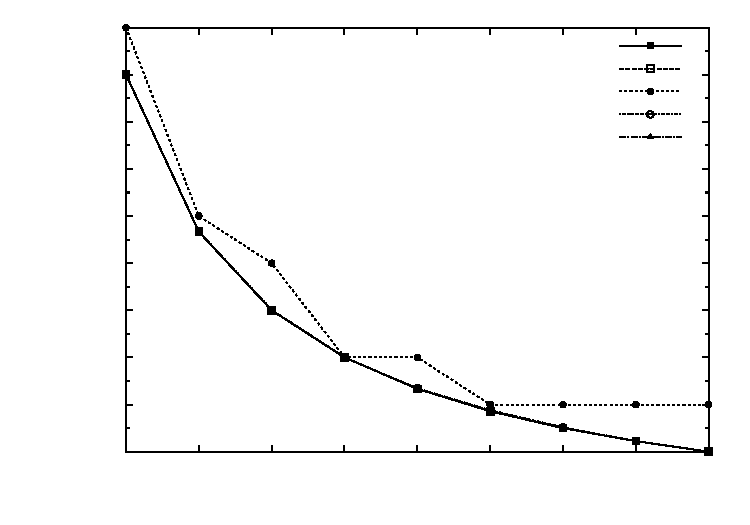
\includegraphics{graph_balance}}%
    \gplfronttext
  \end{picture}%
\endgroup
}
}
\hfill
\subfigure[Edgecut]{
\label{fig:graph-edgecut}
\scalebox{.5}{% GNUPLOT: LaTeX picture with Postscript
\begingroup
  \makeatletter
  \providecommand\color[2][]{%
    \GenericError{(gnuplot) \space\space\space\@spaces}{%
      Package color not loaded in conjunction with
      terminal option `colourtext'%
    }{See the gnuplot documentation for explanation.%
    }{Either use 'blacktext' in gnuplot or load the package
      color.sty in LaTeX.}%
    \renewcommand\color[2][]{}%
  }%
  \providecommand\includegraphics[2][]{%
    \GenericError{(gnuplot) \space\space\space\@spaces}{%
      Package graphicx or graphics not loaded%
    }{See the gnuplot documentation for explanation.%
    }{The gnuplot epslatex terminal needs graphicx.sty or graphics.sty.}%
    \renewcommand\includegraphics[2][]{}%
  }%
  \providecommand\rotatebox[2]{#2}%
  \@ifundefined{ifGPcolor}{%
    \newif\ifGPcolor
    \GPcolorfalse
  }{}%
  \@ifundefined{ifGPblacktext}{%
    \newif\ifGPblacktext
    \GPblacktexttrue
  }{}%
  % define a \g@addto@macro without @ in the name:
  \let\gplgaddtomacro\g@addto@macro
  % define empty templates for all commands taking text:
  \gdef\gplbacktext{}%
  \gdef\gplfronttext{}%
  \makeatother
  \ifGPblacktext
    % no textcolor at all
    \def\colorrgb#1{}%
    \def\colorgray#1{}%
  \else
    % gray or color?
    \ifGPcolor
      \def\colorrgb#1{\color[rgb]{#1}}%
      \def\colorgray#1{\color[gray]{#1}}%
      \expandafter\def\csname LTw\endcsname{\color{white}}%
      \expandafter\def\csname LTb\endcsname{\color{black}}%
      \expandafter\def\csname LTa\endcsname{\color{black}}%
      \expandafter\def\csname LT0\endcsname{\color[rgb]{1,0,0}}%
      \expandafter\def\csname LT1\endcsname{\color[rgb]{0,1,0}}%
      \expandafter\def\csname LT2\endcsname{\color[rgb]{0,0,1}}%
      \expandafter\def\csname LT3\endcsname{\color[rgb]{1,0,1}}%
      \expandafter\def\csname LT4\endcsname{\color[rgb]{0,1,1}}%
      \expandafter\def\csname LT5\endcsname{\color[rgb]{1,1,0}}%
      \expandafter\def\csname LT6\endcsname{\color[rgb]{0,0,0}}%
      \expandafter\def\csname LT7\endcsname{\color[rgb]{1,0.3,0}}%
      \expandafter\def\csname LT8\endcsname{\color[rgb]{0.5,0.5,0.5}}%
    \else
      % gray
      \def\colorrgb#1{\color{black}}%
      \def\colorgray#1{\color[gray]{#1}}%
      \expandafter\def\csname LTw\endcsname{\color{white}}%
      \expandafter\def\csname LTb\endcsname{\color{black}}%
      \expandafter\def\csname LTa\endcsname{\color{black}}%
      \expandafter\def\csname LT0\endcsname{\color{black}}%
      \expandafter\def\csname LT1\endcsname{\color{black}}%
      \expandafter\def\csname LT2\endcsname{\color{black}}%
      \expandafter\def\csname LT3\endcsname{\color{black}}%
      \expandafter\def\csname LT4\endcsname{\color{black}}%
      \expandafter\def\csname LT5\endcsname{\color{black}}%
      \expandafter\def\csname LT6\endcsname{\color{black}}%
      \expandafter\def\csname LT7\endcsname{\color{black}}%
      \expandafter\def\csname LT8\endcsname{\color{black}}%
    \fi
  \fi
  \setlength{\unitlength}{0.0500bp}%
  \begin{picture}(7200.00,5040.00)%
    \gplgaddtomacro\gplbacktext{%
      \csname LTb\endcsname%
      \put(946,704){\makebox(0,0)[r]{\strut{} 0}}%
      \put(946,1136){\makebox(0,0)[r]{\strut{} 0.1}}%
      \put(946,1568){\makebox(0,0)[r]{\strut{} 0.2}}%
      \put(946,2000){\makebox(0,0)[r]{\strut{} 0.3}}%
      \put(946,2432){\makebox(0,0)[r]{\strut{} 0.4}}%
      \put(946,2865){\makebox(0,0)[r]{\strut{} 0.5}}%
      \put(946,3297){\makebox(0,0)[r]{\strut{} 0.6}}%
      \put(946,3729){\makebox(0,0)[r]{\strut{} 0.7}}%
      \put(946,4161){\makebox(0,0)[r]{\strut{} 0.8}}%
      \put(946,4593){\makebox(0,0)[r]{\strut{} 0.9}}%
      \put(1078,484){\makebox(0,0){\strut{} 2}}%
      \put(1794,484){\makebox(0,0){\strut{} 3}}%
      \put(2509,484){\makebox(0,0){\strut{} 4}}%
      \put(3225,484){\makebox(0,0){\strut{} 5}}%
      \put(3941,484){\makebox(0,0){\strut{} 6}}%
      \put(4656,484){\makebox(0,0){\strut{} 7}}%
      \put(5372,484){\makebox(0,0){\strut{} 8}}%
      \put(6087,484){\makebox(0,0){\strut{} 9}}%
      \put(6803,484){\makebox(0,0){\strut{} 10}}%
      \put(176,2739){\rotatebox{-270}{\makebox(0,0){\strut{}\% edgecut }}}%
      \put(3940,154){\makebox(0,0){\strut{}\# of partitions}}%
    }%
    \gplgaddtomacro\gplfronttext{%
      \csname LTb\endcsname%
      \put(5805,2755){\makebox(0,0)[r]{\strut{}\bunny}}%
      \csname LTb\endcsname%
      \put(5805,2535){\makebox(0,0)[r]{\strut{}\blobs}}%
      \csname LTb\endcsname%
      \put(5805,2315){\makebox(0,0)[r]{\strut{}\clique}}%
      \csname LTb\endcsname%
      \put(5805,2095){\makebox(0,0)[r]{\strut{}\gnp}}%
      \csname LTb\endcsname%
      \put(5805,1875){\makebox(0,0)[r]{\strut{}\sphere}}%
    }%
    \gplbacktext
    \put(0,0){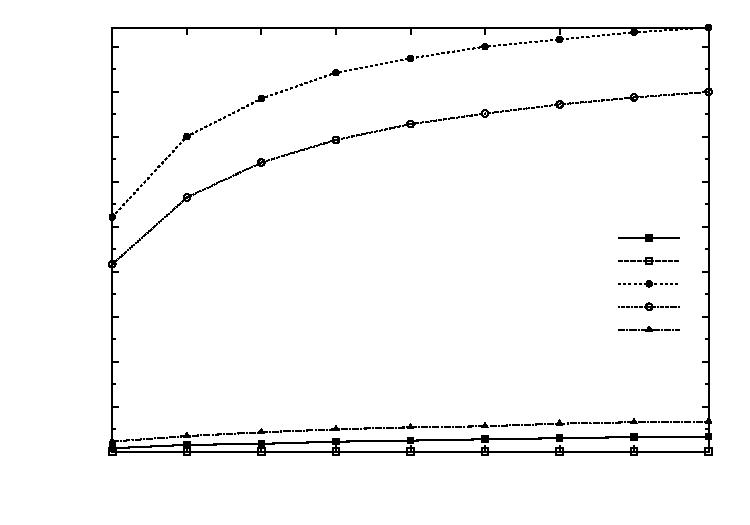
\includegraphics{edgecut}}%
    \gplfronttext
  \end{picture}%
\endgroup
}
}
\caption{Edgecut and balance ratios computed on the 1-skeleton of each dataset.} 
\end{figure*}

\begin{figure*}
\centering
\subfigure[Blowup Factor $\factor$]{
\label{fig:blowup-factors}
\scalebox{.5}{% GNUPLOT: LaTeX picture with Postscript
\begingroup
  \makeatletter
  \providecommand\color[2][]{%
    \GenericError{(gnuplot) \space\space\space\@spaces}{%
      Package color not loaded in conjunction with
      terminal option `colourtext'%
    }{See the gnuplot documentation for explanation.%
    }{Either use 'blacktext' in gnuplot or load the package
      color.sty in LaTeX.}%
    \renewcommand\color[2][]{}%
  }%
  \providecommand\includegraphics[2][]{%
    \GenericError{(gnuplot) \space\space\space\@spaces}{%
      Package graphicx or graphics not loaded%
    }{See the gnuplot documentation for explanation.%
    }{The gnuplot epslatex terminal needs graphicx.sty or graphics.sty.}%
    \renewcommand\includegraphics[2][]{}%
  }%
  \providecommand\rotatebox[2]{#2}%
  \@ifundefined{ifGPcolor}{%
    \newif\ifGPcolor
    \GPcolorfalse
  }{}%
  \@ifundefined{ifGPblacktext}{%
    \newif\ifGPblacktext
    \GPblacktexttrue
  }{}%
  % define a \g@addto@macro without @ in the name:
  \let\gplgaddtomacro\g@addto@macro
  % define empty templates for all commands taking text:
  \gdef\gplbacktext{}%
  \gdef\gplfronttext{}%
  \makeatother
  \ifGPblacktext
    % no textcolor at all
    \def\colorrgb#1{}%
    \def\colorgray#1{}%
  \else
    % gray or color?
    \ifGPcolor
      \def\colorrgb#1{\color[rgb]{#1}}%
      \def\colorgray#1{\color[gray]{#1}}%
      \expandafter\def\csname LTw\endcsname{\color{white}}%
      \expandafter\def\csname LTb\endcsname{\color{black}}%
      \expandafter\def\csname LTa\endcsname{\color{black}}%
      \expandafter\def\csname LT0\endcsname{\color[rgb]{1,0,0}}%
      \expandafter\def\csname LT1\endcsname{\color[rgb]{0,1,0}}%
      \expandafter\def\csname LT2\endcsname{\color[rgb]{0,0,1}}%
      \expandafter\def\csname LT3\endcsname{\color[rgb]{1,0,1}}%
      \expandafter\def\csname LT4\endcsname{\color[rgb]{0,1,1}}%
      \expandafter\def\csname LT5\endcsname{\color[rgb]{1,1,0}}%
      \expandafter\def\csname LT6\endcsname{\color[rgb]{0,0,0}}%
      \expandafter\def\csname LT7\endcsname{\color[rgb]{1,0.3,0}}%
      \expandafter\def\csname LT8\endcsname{\color[rgb]{0.5,0.5,0.5}}%
    \else
      % gray
      \def\colorrgb#1{\color{black}}%
      \def\colorgray#1{\color[gray]{#1}}%
      \expandafter\def\csname LTw\endcsname{\color{white}}%
      \expandafter\def\csname LTb\endcsname{\color{black}}%
      \expandafter\def\csname LTa\endcsname{\color{black}}%
      \expandafter\def\csname LT0\endcsname{\color{black}}%
      \expandafter\def\csname LT1\endcsname{\color{black}}%
      \expandafter\def\csname LT2\endcsname{\color{black}}%
      \expandafter\def\csname LT3\endcsname{\color{black}}%
      \expandafter\def\csname LT4\endcsname{\color{black}}%
      \expandafter\def\csname LT5\endcsname{\color{black}}%
      \expandafter\def\csname LT6\endcsname{\color{black}}%
      \expandafter\def\csname LT7\endcsname{\color{black}}%
      \expandafter\def\csname LT8\endcsname{\color{black}}%
    \fi
  \fi
  \setlength{\unitlength}{0.0500bp}%
  \begin{picture}(7200.00,5040.00)%
    \gplgaddtomacro\gplbacktext{%
      \csname LTb\endcsname%
      \put(1078,704){\makebox(0,0)[r]{\strut{} 1}}%
      \put(1078,1196){\makebox(0,0)[r]{\strut{} 1.05}}%
      \put(1078,1688){\makebox(0,0)[r]{\strut{} 1.1}}%
      \put(1078,2180){\makebox(0,0)[r]{\strut{} 1.15}}%
      \put(1078,2672){\makebox(0,0)[r]{\strut{} 1.2}}%
      \put(1078,3165){\makebox(0,0)[r]{\strut{} 1.25}}%
      \put(1078,3657){\makebox(0,0)[r]{\strut{} 1.3}}%
      \put(1078,4149){\makebox(0,0)[r]{\strut{} 1.35}}%
      \put(1078,4641){\makebox(0,0)[r]{\strut{} 1.4}}%
      \put(1210,484){\makebox(0,0){\strut{} 2}}%
      \put(1909,484){\makebox(0,0){\strut{} 3}}%
      \put(2608,484){\makebox(0,0){\strut{} 4}}%
      \put(3307,484){\makebox(0,0){\strut{} 5}}%
      \put(4007,484){\makebox(0,0){\strut{} 6}}%
      \put(4706,484){\makebox(0,0){\strut{} 7}}%
      \put(5405,484){\makebox(0,0){\strut{} 8}}%
      \put(6104,484){\makebox(0,0){\strut{} 9}}%
      \put(6803,484){\makebox(0,0){\strut{} 10}}%
      \put(176,2739){\rotatebox{-270}{\makebox(0,0){\strut{}blowup factor }}}%
      \put(4006,154){\makebox(0,0){\strut{}\# of partitions}}%
    }%
    \gplgaddtomacro\gplfronttext{%
      \csname LTb\endcsname%
      \put(5816,4602){\makebox(0,0)[r]{\strut{}\bunny}}%
      \csname LTb\endcsname%
      \put(5816,4382){\makebox(0,0)[r]{\strut{}\blobs}}%
      \csname LTb\endcsname%
      \put(5816,4162){\makebox(0,0)[r]{\strut{}\clique}}%
      \csname LTb\endcsname%
      \put(5816,3942){\makebox(0,0)[r]{\strut{}\gnp}}%
      \csname LTb\endcsname%
      \put(5816,3722){\makebox(0,0)[r]{\strut{}\sphere}}%
    }%
    \gplbacktext
    \put(0,0){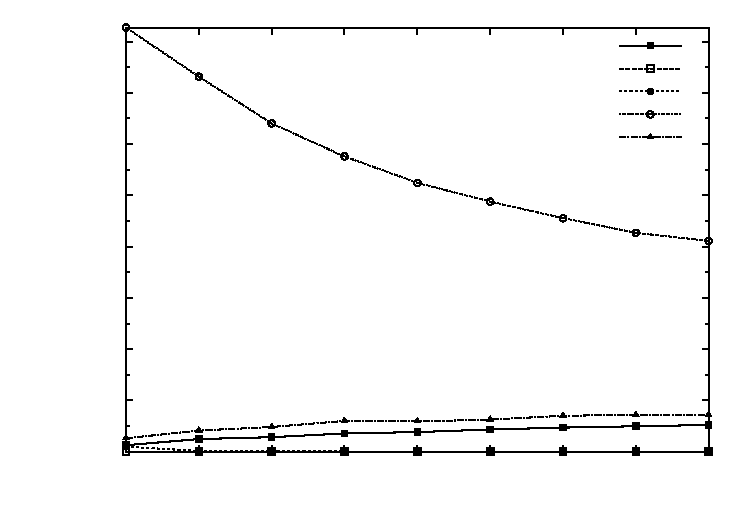
\includegraphics{blowup-factors}}%
    \gplfronttext
  \end{picture}%
\endgroup
}
}
\subfigure[Balance Ratio $\alpha$ for each covering]{
\label{fig:balance-factors}
\scalebox{.5}{% GNUPLOT: LaTeX picture with Postscript
\begingroup
  \makeatletter
  \providecommand\color[2][]{%
    \GenericError{(gnuplot) \space\space\space\@spaces}{%
      Package color not loaded in conjunction with
      terminal option `colourtext'%
    }{See the gnuplot documentation for explanation.%
    }{Either use 'blacktext' in gnuplot or load the package
      color.sty in LaTeX.}%
    \renewcommand\color[2][]{}%
  }%
  \providecommand\includegraphics[2][]{%
    \GenericError{(gnuplot) \space\space\space\@spaces}{%
      Package graphicx or graphics not loaded%
    }{See the gnuplot documentation for explanation.%
    }{The gnuplot epslatex terminal needs graphicx.sty or graphics.sty.}%
    \renewcommand\includegraphics[2][]{}%
  }%
  \providecommand\rotatebox[2]{#2}%
  \@ifundefined{ifGPcolor}{%
    \newif\ifGPcolor
    \GPcolorfalse
  }{}%
  \@ifundefined{ifGPblacktext}{%
    \newif\ifGPblacktext
    \GPblacktexttrue
  }{}%
  % define a \g@addto@macro without @ in the name:
  \let\gplgaddtomacro\g@addto@macro
  % define empty templates for all commands taking text:
  \gdef\gplbacktext{}%
  \gdef\gplfronttext{}%
  \makeatother
  \ifGPblacktext
    % no textcolor at all
    \def\colorrgb#1{}%
    \def\colorgray#1{}%
  \else
    % gray or color?
    \ifGPcolor
      \def\colorrgb#1{\color[rgb]{#1}}%
      \def\colorgray#1{\color[gray]{#1}}%
      \expandafter\def\csname LTw\endcsname{\color{white}}%
      \expandafter\def\csname LTb\endcsname{\color{black}}%
      \expandafter\def\csname LTa\endcsname{\color{black}}%
      \expandafter\def\csname LT0\endcsname{\color[rgb]{1,0,0}}%
      \expandafter\def\csname LT1\endcsname{\color[rgb]{0,1,0}}%
      \expandafter\def\csname LT2\endcsname{\color[rgb]{0,0,1}}%
      \expandafter\def\csname LT3\endcsname{\color[rgb]{1,0,1}}%
      \expandafter\def\csname LT4\endcsname{\color[rgb]{0,1,1}}%
      \expandafter\def\csname LT5\endcsname{\color[rgb]{1,1,0}}%
      \expandafter\def\csname LT6\endcsname{\color[rgb]{0,0,0}}%
      \expandafter\def\csname LT7\endcsname{\color[rgb]{1,0.3,0}}%
      \expandafter\def\csname LT8\endcsname{\color[rgb]{0.5,0.5,0.5}}%
    \else
      % gray
      \def\colorrgb#1{\color{black}}%
      \def\colorgray#1{\color[gray]{#1}}%
      \expandafter\def\csname LTw\endcsname{\color{white}}%
      \expandafter\def\csname LTb\endcsname{\color{black}}%
      \expandafter\def\csname LTa\endcsname{\color{black}}%
      \expandafter\def\csname LT0\endcsname{\color{black}}%
      \expandafter\def\csname LT1\endcsname{\color{black}}%
      \expandafter\def\csname LT2\endcsname{\color{black}}%
      \expandafter\def\csname LT3\endcsname{\color{black}}%
      \expandafter\def\csname LT4\endcsname{\color{black}}%
      \expandafter\def\csname LT5\endcsname{\color{black}}%
      \expandafter\def\csname LT6\endcsname{\color{black}}%
      \expandafter\def\csname LT7\endcsname{\color{black}}%
      \expandafter\def\csname LT8\endcsname{\color{black}}%
    \fi
  \fi
  \setlength{\unitlength}{0.0500bp}%
  \begin{picture}(7200.00,5040.00)%
    \gplgaddtomacro\gplbacktext{%
      \csname LTb\endcsname%
      \put(946,704){\makebox(0,0)[r]{\strut{} 0.1}}%
      \put(946,1156){\makebox(0,0)[r]{\strut{} 0.2}}%
      \put(946,1609){\makebox(0,0)[r]{\strut{} 0.3}}%
      \put(946,2061){\makebox(0,0)[r]{\strut{} 0.4}}%
      \put(946,2513){\makebox(0,0)[r]{\strut{} 0.5}}%
      \put(946,2966){\makebox(0,0)[r]{\strut{} 0.6}}%
      \put(946,3418){\makebox(0,0)[r]{\strut{} 0.7}}%
      \put(946,3870){\makebox(0,0)[r]{\strut{} 0.8}}%
      \put(946,4323){\makebox(0,0)[r]{\strut{} 0.9}}%
      \put(946,4775){\makebox(0,0)[r]{\strut{} 1}}%
      \put(1078,484){\makebox(0,0){\strut{} 2}}%
      \put(1794,484){\makebox(0,0){\strut{} 3}}%
      \put(2509,484){\makebox(0,0){\strut{} 4}}%
      \put(3225,484){\makebox(0,0){\strut{} 5}}%
      \put(3941,484){\makebox(0,0){\strut{} 6}}%
      \put(4656,484){\makebox(0,0){\strut{} 7}}%
      \put(5372,484){\makebox(0,0){\strut{} 8}}%
      \put(6087,484){\makebox(0,0){\strut{} 9}}%
      \put(6803,484){\makebox(0,0){\strut{} 10}}%
      \put(176,2739){\rotatebox{-270}{\makebox(0,0){\strut{}balance ratio}}}%
      \put(3940,154){\makebox(0,0){\strut{}\# of partitions}}%
    }%
    \gplgaddtomacro\gplfronttext{%
      \csname LTb\endcsname%
      \put(5805,2403){\makebox(0,0)[r]{\strut{}\bunny}}%
      \csname LTb\endcsname%
      \put(5805,2183){\makebox(0,0)[r]{\strut{}\blobs}}%
      \csname LTb\endcsname%
      \put(5805,1963){\makebox(0,0)[r]{\strut{}\clique}}%
      \csname LTb\endcsname%
      \put(5805,1743){\makebox(0,0)[r]{\strut{}\gnp}}%
      \csname LTb\endcsname%
      \put(5805,1523){\makebox(0,0)[r]{\strut{}\sphere}}%
    }%
    \gplbacktext
    \put(0,0){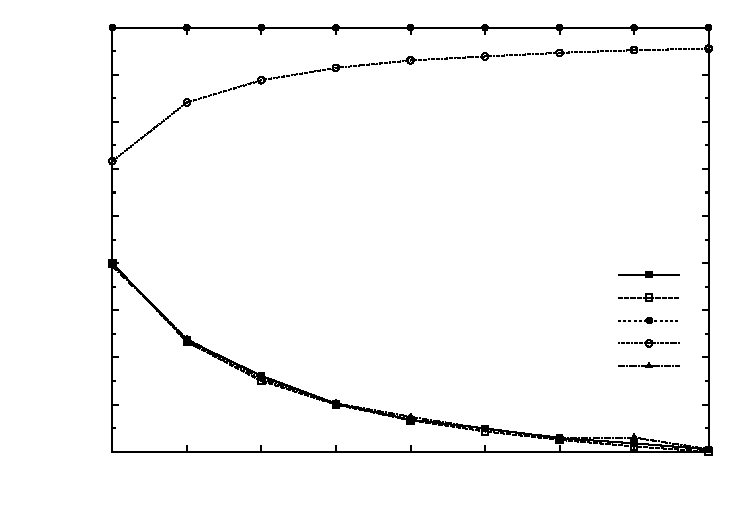
\includegraphics{balance-factors}}%
    \gplfronttext
  \end{picture}%
\endgroup
}
}
\caption{Blowup factor and cover balance ratio for each complex.}
\end{figure*}
 
\subsection{Timing}
\begin{figure}[h]
\centering
\begin{subfigure}[b]{.45\textwidth}
\centering
\begin{tikzpicture}[scale=.65]
\begin{axis}[xlabel=\# of partitions, minor y tick num={1}, ylabel=speedup factor, legend style={legend pos=north west, font=\small}]
\legend{\multiblob, \bunny, \clique, \gnp, \sphere, ideal}
\addplot table [x=num_partitions, skip coords between index={0}{1}, y=speedup, col sep=comma, ignore chars=']
{pgf-speedup-figs/results/concurrent_homology/clique.11.22720.csv};
\addplot table [x=num_partitions, skip coords between index={0}{1}, y=speedup, col sep=comma, ignore chars=']
{pgf-speedup-figs/results/concurrent_homology/bunny..05.csv};
\addplot table [x=num_partitions, skip coords between index={0}{1}, y=speedup, col sep=comma, ignore chars=']
{pgf-speedup-figs/results/concurrent_homology/clique.20.csv};
\addplot table [x=num_partitions, skip coords between index={0}{1}, y=speedup, col sep=comma, ignore chars=']
{pgf-speedup-figs/results/concurrent_homology/gnp.1250.047.csv};
\addplot table [x=num_partitions, skip coords between index={0}{1}, y=speedup, col sep=comma, ignore chars=']
{pgf-speedup-figs/results/concurrent_homology/sphere.csv};
\addplot[dash pattern=on 4pt off 1pt on 4pt off 4pt, domain=2:10]{x+1};
\end{axis}
\end{tikzpicture}
\caption{Speedup factor for reducing $\partial_{\K^{\C}}$}
\label{fig:blowup-homology-speedup}
\end{subfigure}
\hfill
\begin{subfigure}[b]{.45\textwidth}
\centering
\begin{tikzpicture}[scale=.65]
%\pgfplotsset{ymax=5}
\begin{axis}[xlabel=\# of partitions/threads, minor y tick num={1}, ylabel=speedup factor, legend style={legend pos=north west, font=\small}]
\legend{\multiblob, \bunny, \clique, \gnp, \sphere, ideal}
\addplot table [x=num_partitions, skip coords between index={0}{1}, y=speedup, col sep=comma, ignore chars=']
{pgf-speedup-figs/results/cover_homology/clique.11.22720.csv};
\addplot table [x=num_partitions, skip coords between index={0}{1}, y=speedup, col sep=comma, ignore chars=']
{pgf-speedup-figs/results/cover_homology/bunny..05.csv};
\addplot table [x=num_partitions, skip coords between index={0}{1}, y=speedup, col sep=comma, ignore chars=']
{pgf-speedup-figs/results/cover_homology/clique.20.csv};
\addplot table [x=num_partitions, skip coords between index={0}{1}, y=speedup, col sep=comma, ignore chars=']
{pgf-speedup-figs/results/cover_homology/gnp.1250.047.csv};
\addplot table [x=num_partitions, skip coords between index={0}{1}, y=speedup, col sep=comma, ignore chars=']
{pgf-speedup-figs/results/cover_homology/sphere.csv};
\addplot[dash pattern=on 4pt off 1pt on 4pt off 4pt, domain=2:10]{x};
\end{axis}
\end{tikzpicture}
\caption{Speedup factor for reducing $\partial_{\K}$}
\label{fig:nonblowup-homology-speedup}
\end{subfigure}
\caption{(Left) Speedup factor $T_s/T_p$ where $T_p$ is the time to reduce $\partial_{\K^\C}$ in parallel on $p+1$ threads  and $T_s$ is the time to reduce $\partial_K$ in serial. (Right) Speedup factor of $T_s/T_p$ where $T_p$ measures the time to reduce $\partial_{\K}$ in parallel.}
\label{fig:reduction-speedup}
\end{figure}
For each of our data sets we present the speedup factor of
our algorithm versus serial persistence. Figure~\ref{fig:total-speedup}
shows the speedup factor of our entire algorithm from start to finish as 
compared to a persistence run in serial on the same input, from start to 
finish. In Figure~\ref{fig:homology-speedup} we also compare the speedup for 
homology computations between both algorithms.

First, we can see that our techniques tend to scale the best on inputs
in which all topological features are localized by the cover. However we see significantly 
better performance on $\bunny$ versus $\blobs$. Due to the massive size
of each $\blobs$, we believe that the variation between these two experiments is 
demonstrating how memory bandwidth does not scale with the number
of cores used by an algorithm. One might consider mitigating the effect of limited memory 
bandwith by prefetching or other architecture specific parallelization
techniques, but our goal is to demonstrate proof of concept, not optimization for all cases.

Second, geometric inputs such as a $\sphere$ have entirely global topology; these
features are necessarily resolved by a long serial computation. However, they still
emit a balanced cover, so the bulk of the work is still evenly divided across each core,
and we still see a linear speedup on this input.
 
Finally, we see that inputs such as $\clique$ or $\gnp$ which are flag complexes of cliques or
expander complexes, have entirely global topological structure,
emit no balanced cover. and produce a small blowup factor. 
Our algorithm is slower than the equivalent serial computations which
is expected.